\documentclass[a4paper]{article}

\usepackage{ngerman}
\usepackage{a4wide}
\usepackage{graphicx}
\usepackage[utf8]{inputenc}
\usepackage{amscd}
\usepackage{amssymb}
\usepackage{amsmath}
\usepackage{bibgerm}
\usepackage{hyperref}
\usepackage{gensymb}
\usepackage[section]{placeins}
\usepackage[export]{adjustbox}
\usepackage{listings}
\lstset{
	 literate={ö}{{\"o}}1 	%Replaces "oe","ae" usw. with \o to use "Umlaute" in listings
           {ä}{{\"a}}1
           {ü}{{\"u}}1
	{ß}{{\ss}}1
	{=}{$\rightarrow{}$}{1},
  	breaklines=true,                % sets automatic line breaking
	columns=flexible
}

\graphicspath{{./Kapitel/img/}}

%%%
%%% Style-Definition des Literaturverzeichnis
%%%
%%

\bibliographystyle{alpha}
\bibliographystyle{geralpha}
 
%%\setlength{\parindent}{0pt} %kein Einzug beim Absatzbegin
\setlength{\parskip}\medskipamount %Abstand zwischen 2 Abs�tzen
\setcounter{tocdepth}{4} 
\setcounter{secnumdepth}{4}

\author{Matthias Kemmer, Julius Hackel, Markus Bullmann, Stefan Gerasch}
\title{Gliederung Vertiefungsseminar MI}
\begin{document}

\maketitle
\tableofcontents

\newpage
\section{Einführung}
Die \textbf{Frequenzmodulationssynthese} ist eine für die Musikwelt sehr wichtige Anwendung der \textbf{Frequenzmodulation (FM)}, welche bereits aus der Nachrichtentechnik bekannt ist. Eine Motivation für diese Seminararbeit ist die Tatsache, dass die Musikwelt durch FM-Synthese eine Revolution erlebt hat und ohne diese Erfindung eine Vielzahl an Synthesizern niemals entstanden wäre. Die Arbeit ist im Rahmen des Vertiefungsseminars I der Vertiefung Medieninformatik an der Hochschule für angewandte Wissenschaften Würzburg-Schweinfurt entstanden. %WIP, wer bock hat mag sich was besseres ausdenken :D
\FloatBarrier
\subsection{Prinzip der FM-Synthese}
\label{PrinzipFM}
Generell wird bei der Frequenzmodulation die Frequenz eines \textbf{Trägersignals} durch ein weiteres \textbf{Modulationssignal} verändert, die Amplitude bleibt jedoch unangetastet. In der Nachrichtentechnik können durch die unterschiedlichen Frequenzen im modulierten Träger Informationen übertragen werden. Bei der FM-Synthese kann die maximale Amplitude in besonderen Fällen jedoch von der maximalen Auslenkung des Trägers abweichen bzw. kleiner als diese werden. 
Die momentane Amplitude der Modulation lässt sich bei der FM-Synthese durch folgende Formel beschreiben:
\[
e(t) = A\sin(\alpha t + I\sin(\beta t)) \cite{chowningPaper}
\]
Bei der äußeren Sinusfunktion handelt es sich um den Träger, welcher in seiner Frequenz durch das Modulationssignal (innerer Sinus) moduliert wird.

\textbf{Abbildung \ref{fig:vergleichSignale}} veranschaulicht die Frequenzmodulation eines Trägers durch den Modulator.

\begin{figure} [ht]
\centering
  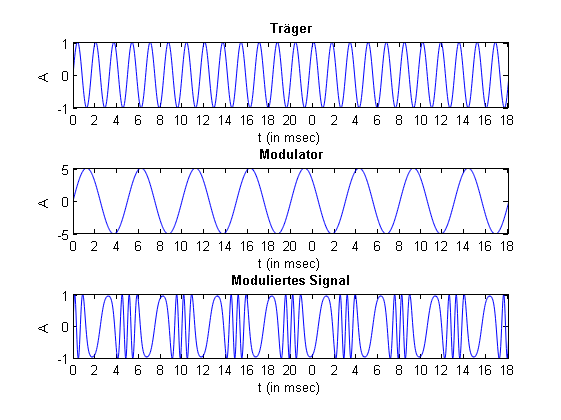
\includegraphics[width=0.95\textwidth]{Prinzip.png}
\caption{Vergleich Träger/Modulator}
\label{fig:vergleichSignale}
\end{figure}
\FloatBarrier

Technisch gesehen kann die FM-Synthese mit Oszillatoren umgesetzt werden. In der einfachsten Form benötigt man dazu einen Träger-Oszillator und einen Modulator-Oszillator. Wie eine einfache FM-Synthese in Form einer Schaltung aussehen kann, zeigt Abbildung \textbf{Abbildung \ref{fig:schaltung}}. Der Ausgang des ersten Oszillators geht dabei in den Eingang des Zweiten. Dabei kann entweder direkt die Frequenz des Trägers beeinflusst werden, jedoch auch dessen Phase. Bei VCA handelt es sich um einen spannungsgesteuerten Verstärker (Voltage controlled amplifier), EG ist ein Hüllkurvengenerator (Envelope Generator). $f_M$ und $f_C$ sind die Frequenzen der beiden Oszillatoren. Über den Modulationsindex $\beta$ kann die Sträke der Modulation festgelegt werden. 

\begin{figure} [ht]
\centering
  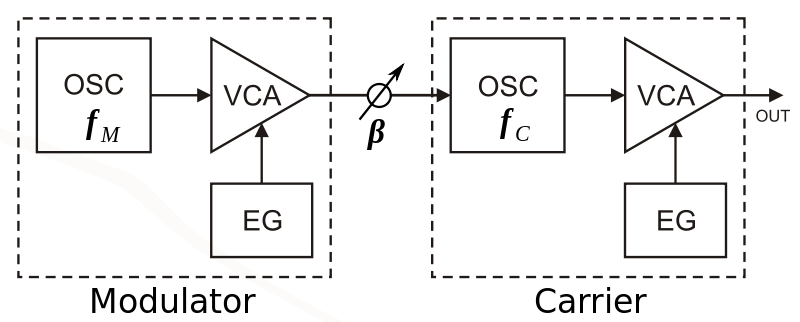
\includegraphics[width=0.8\textwidth,frame]{schaltung.png}
\caption{Abbildung einer einfachen FM-Synthese als Schaltung}
\label{fig:schaltung}
Quelle: \url{http://mmmmaven.com/wp-content/uploads/800px-2op_FM.svg_.png} 
\\Stand 16.06.2015
\end{figure}

Die Frequenzmodulationssynthese ist in ihren Grundzügen recht einfach zu verstehen. Es können mit geringem Aufwand bereits sehr komplexe, wenn auch oft unkontrollierbare, Signale mit komplexen Klangspektren (bzw. Frequenzspektren) erzeugen. Wie sich im Folgenden jedoch noch herausstellen wird, ist es dagegen sehr schwierig, durch die FM-Synthese gezielt Signale zu erzeugen und diese zu kontrollieren.

Praktisch gesehen kann die Frequenzmodulationssynthese dazu verwendet werden, um Klangbilder echter Instrumente nachzubilden, jedoch auch für die Erzeugung ganz neuer Töne, die so nicht in der Natur vorkommen.

\FloatBarrier
\subsection{Beispiele}
In diesem Kapitel werden einige konkrete Beispiele der FM-Synthese anhand von Träger- und Modulationssignal sowie der daraus resultierenden Signals aufgezeigt. Die Grafiken zeigen jeweils Plots von allen drei Signalen, welche mit MATLAB erzeugt wurden.
Die Frequenzen der jeweiligen Funktionen wurden so gewählt, dass sie in einem Frequenzbereich liegen der vom menschlichen Ohr wahrgenommen werden kann. (siehe Unterkapitel \textbf{``\ref{bulli:ohrToeneUndFrequenzen} - \nameref{bulli:ohrToeneUndFrequenzen}''}).

\begin{figure} [ht]
\centering
  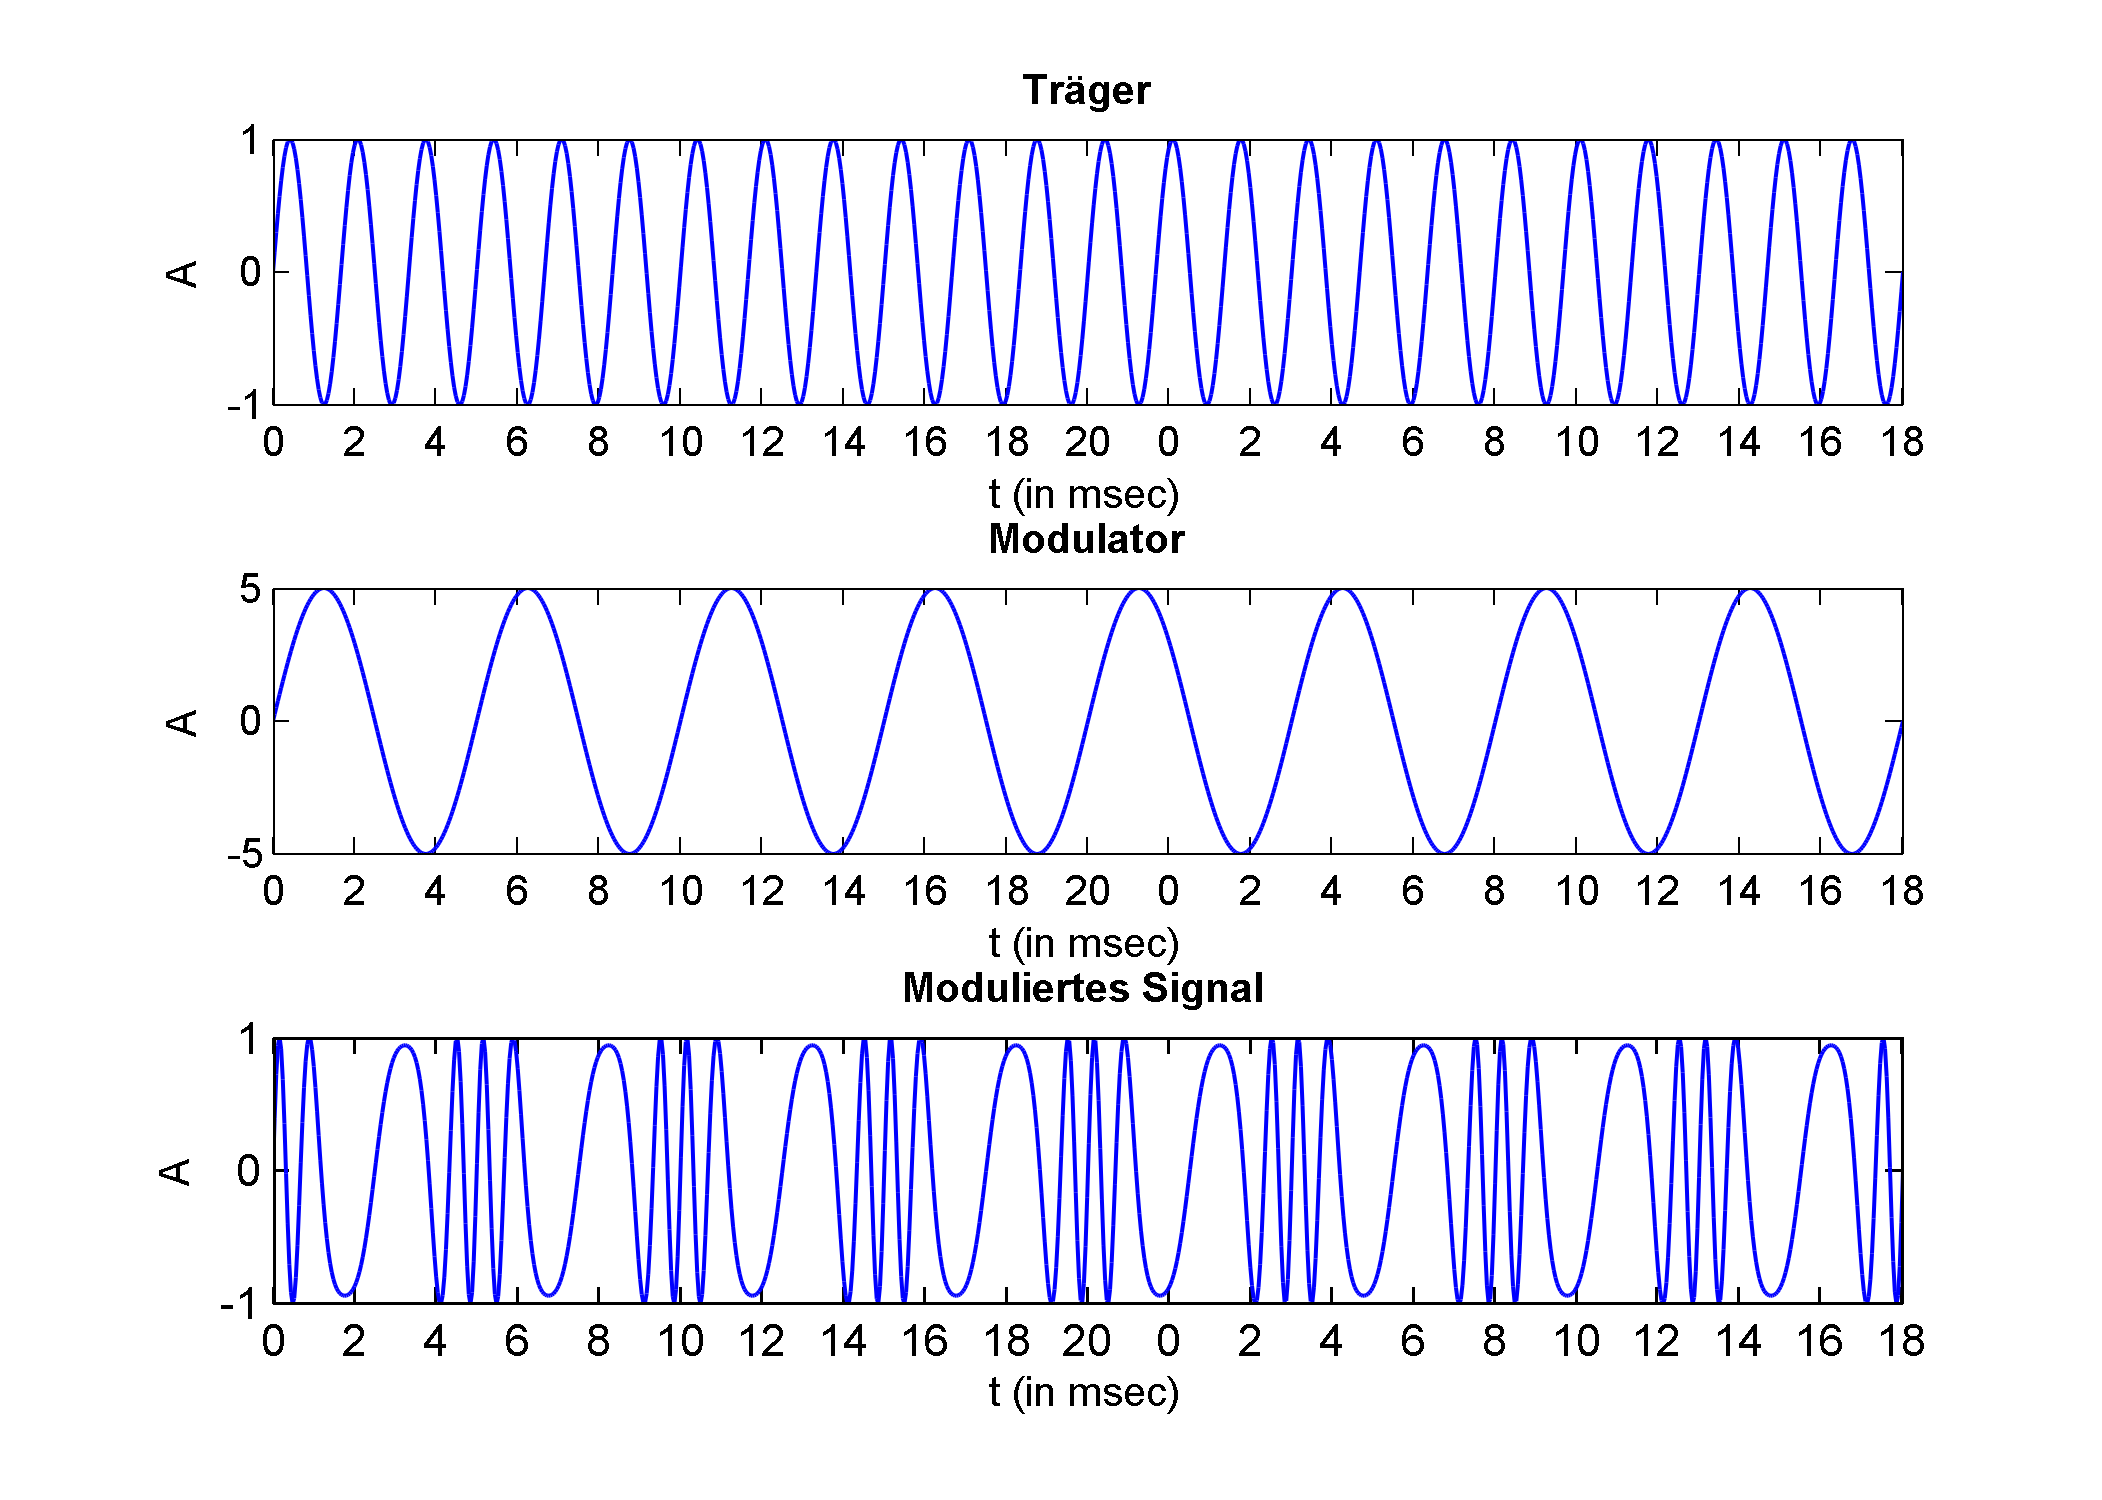
\includegraphics[width=0.95\textwidth]{Beispiel1.png}
\caption{Beispiel 1. Darstellung einer Frequenzmodulation mit einer Trägerfrequenz von 600 Hz, einer Modulationsfrequenz von 75 Hz und einem Modulationsindex von 5 }
\label{fig:beispiel1}
\end{figure}

In Beispiel 1 (siehe \textbf{Abbildung \ref{fig:beispiel1}})  wurden folgende Signale verwendet:

\begin{lstlisting}[mathescape]
Trägersignal: 		$y(t) = \,\;\;\sin(2 \pi 600\cdot t)$
Modulator:		$y(t) =5 \sin(2 \pi 75\cdot t)$
Gesamtfunktion: 	$y(t) = \,\;\;\sin(2 \pi 600\cdot t + 5 \sin(2 \pi 75\cdot t))$
\end{lstlisting}

Konkret bedeuted eine Trägerfrequenz von 600 Hz, dass die Trägerfunktion 600 mal in der Sekunde schwingt, d.h. eine Periode ist genau $\frac{1}{600}$ Sekunden lang. Der Modulator hat eine Frequenz von 75 Hz, wodurch er 75 Schwingung pro Sekunde durchläuft und eine Periode dann $\frac{1}{75}$ Sekunden lang ist. Für die Modulation gilt im Allgemeinen, dass der sogenannte Frequenzhub der Modulation (Erklärung siehe Kapitel \textbf{``\ref{chowningparameter} - \nameref{chowningparameter}''}) immer dann Maximal ist, wenn die Änderung der Modulationsfunktion (also deren Steigung) ihr Maximum bzw. Minimum hat. In der Grafik tritt dies immer dann auf, wenn der Modulator den Funktionswert 0 hat.

\begin{figure} [ht]
\centering
  \includegraphics[width=0.95\textwidth]{Beispiel2.png}
\caption{Beispiel 2. Darstellung einer Frequenzmodulation mit einer Trägerfrequenz von 300 Hz, einer Modulationsfrequenz von 120 Hz und einem Modulationsindex von 5}
\label{fig:beispiel2}
\end{figure}

Das zweite Beispiel in \textbf{Abbildung \ref{fig:beispiel2}} zeigt eine Frequenzmodulation, bei der sich auch die Amplitude des Signals ändert. Dies geschieht rein durch die Phasenverschiebung des äußeren Sinus durch den Modulator, die tatsächliche Amplitude der Funktion bleibt dabei unangetastet. Die Formel des modulierten Signals sieht wie folgt aus:

\[
y(t) = \sin(2 \pi 300\cdot t + 5 \sin(2 \pi 120\cdot t))
\]

An diesem Beispiel kann man sehr gut erkennen, dass die FM-Synthese mit wenig Aufwand komplexe Signale erzeugen kann, diese jedoch schlecht kontrollierbar bzw. erklärbar sind.

Als gute akustische Beispiele für die Anwendung der FM-Synthese in der Musikwelt können die Stücke \textbf{``Sabelith''} und \textbf{``Turenas'}' von John Chowning, dem Erfinder der FM-Synthese, genannt werden. Beide Stücke wurden ausschließlich mit FM-Synthese erzeugt und beinhalten viele verschiedene Klangarten sowie synthetisierte Instrumente.

\FloatBarrier
\subsection{Geschichte der FM-Synthese}
\label{geschichteFMSynthese}
Die grundlegende Technik hinter der FM-Synthese stammt, wie bereits erwähnt, aus der Nachrichtentechnik. Dort wird das Verfahren ``Frequenzmodulation'' genannt. Prof. Dr. John Chowning selbst gibt als Quelle zu seiner Entdeckung das Buch ``Radio Engineering'' von Frederick Emmons Terman aus dem Jahre 1947 an \cite[S. 35]{soundofinnovation}. Im Jahr 1967 entdeckte John Chowning eine neue Eigenschaft der Frequenzmodulation. Während er mit unterschiedlichen Modulationsfrequenzen experimentierte und dabei verschiedene Vibrato erzeugte, verschwand das Vibrato plötzlich bei höheren Modulationsfrequenzen. Obertöne wurden hörbar, die sich vom eigentlichen Trägersignal abhebten. Unter einem Vibrato versteht man einen schwingenden Ton, d.h. eine pulsierende Änderung der Tonhöhe.\cite{fatherofdigitalmusik}

Chowning selbst war sehr erstaunt über die entstandenen Töne. In einem Interview von 2005 sagte er dazu: 

\textit{``I was experimenting with just a sinusoid and kept increasing the vibrato rate, so all of a sudden it didn't sound like listening to a change in pitch in time, but rather i began to hear timbral differences. So the vibratio became very, very fast, hundreds of times per second, and very, very deep, as if the violinist had a different fingerboard, and the finger was whipping up and down at very high rates and very great distances. That would be sort of a physical metaphor for this.''}\cite[S. 34f.]{soundofinnovation}

Es dauerte 3 Jahre, bis sich Chowning seiner Sache gewiss war und die mathematischen Zusammenhänge ausreichend begründen konnte. Außerdem war er zu diesem Zeitpunkt bereits in der Lage, verschiedene Instrumente wie Trommeln oder Blasinstrumente nachzubilden. Da Chowning selbst leidenschaftlicher Komponist war, veröffentlichte er im Jahre 1971 sein erstes, rein durch FM-Synthese generiertes Stück mit dem Namen ``Sabelithe''. Seine zweite Komposition, ``Turenas'', folgte ein Jahr später.
Um die Stärken seiner neuen Technik zu demonstrieren, verwandelte Chowning beispielsweise in ``Sabelithe'' den Klang einer Trommel in den einer Trompete.\cite[S. 39]{soundofinnovation}
 
\begin{figure} [ht]
\centering
  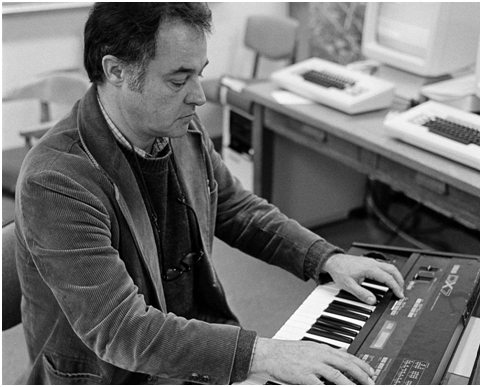
\includegraphics[width=0.8\textwidth]{chowning_CCRMA.png}
\caption{John Chowning am CCRMA}
\label{fig:chowningdx7}
Quelle: \url{ http://arts.mit.edu/wp-content/uploads/2014/07/ChowningYamaha.jpg} \\Stand 09.06.2015
\end{figure}
 
Chowning war, wie auch seine Kollegen, eher Komponist statt Erfinder. Aus diesem Grund waren sie mehr an der musikalischen Seite der Erfindung interessiert als an kommerziellem Erfolg. Obwohl er das Potenzial seiner Erfindung zu dieser Zeit noch nicht überblicken konnte, wendete sich Chowning an das OTL (Office of Technology Licensing) in Stanford. Er hoffte, dass es in der Musikindustrie eine sinnvolle Anwendung seiner Entdeckung gab.\cite[S. 42]{soundofinnovation}

 Zu Beginn war seine Entdeckung jedoch nicht sehr angesehen. Viele der Firmen, welchen das neue Patent angeboten wurde, wussten nichts damit anzufangen und lehnten ab. Andy Moorer, ein Kollege Chownings in Stanford und später Mitgründer des CCRMA, sagte dazu: 

\textit{``[...] It was really discouraging. John was so proud of having put this damn thing together and people didn't really get the idea of spatializing the sound.''}\cite[S. 43]{soundofinnovation}

Offiziell veröffentlichte John Chowning seine neue Entdeckung der Frequenzmodulationssynthese in einem Paper, welches 1973 im ``Journal of the Audio Engineering Society'' unter dem Titel ``The Synthesis of Complex Audio Spectra by Means of Frequenzy Modulation'' erschien.

Erst im Jahr 1974, als ein junger Ingenieur namens Kazukiyo Ishimura von der Firma Yamaha zu einer Vorstellung des Verfahrens geschickt wurde, erkannte dieser binnen wenigen Minuten, welches Potenzial hinter dieser neuen Anwendung der Frequenzmodulation steckt. Yamaha lizensierte das Verfahren noch im gleichen Jahr und Ishimura wurde später Chef des Yamaha Konzerns \cite{fatherofdigitalmusik}.

Im Jahr 1975, nach einiger Zeit Abwesenheit von Stanford, kehrte Chowning dorthin zurück und gründete zusammen mit einigen seiner Kollegen das CCRMA (Center for Computer Research in Music and Acoustics), welches sich auf computergenerierte Musik spezialisiert hat.
Eine Fotografie der Gründer von CCRMA ist auf \textbf{Abbildung \ref{fig:foundersCCRMA}} zu sehen.

\begin{figure} [ht]
\centering
  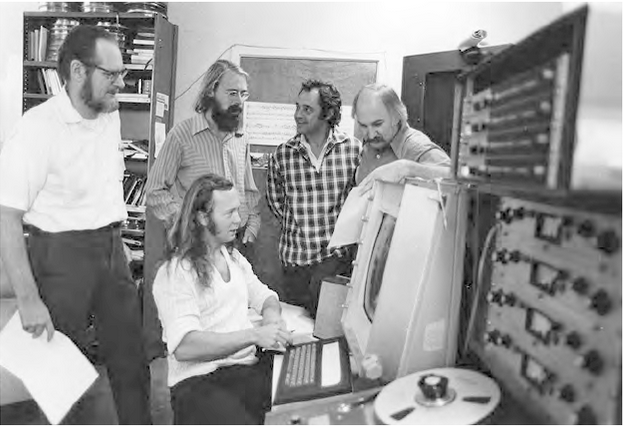
\includegraphics[width=0.8\textwidth]{Founders_CCRMA.png}
\caption{Gründer von CCRMA. Stehend von links nach rechts: Leland Smith, John Grea, John Chowning und Loren Rush. Sitzend: Andy Moorer.}
\label{fig:foundersCCRMA}
Quelle: \cite[S. 52]{soundofinnovation} - Figure 4.1
\end{figure}

Nachdem Yamaha die Technik der FM-Synthese lizenziert hatte, brachte die Firma im Jahre 1980 nach einem Prototypen den ersten digitalen FM-Synthesizer GS1 und zwei Jahre später mit dem GS2 eine kleinere und handlichere Version des GS1 heraus. Die Geräte kosteten um die 30.000 DM für den GS1 bzw. 16.000 DM für den GS2 und waren deshalb nur für ausgewählte Musiker gedacht. Der Durchbruch gelang im Jahre 1983 mit dem DX7. Dieser konnte parallel 16 Stimmen verarbeiten, welche durch 6 sogenannte Operatoren erzeugt wurden. Diese Operatoren waren in 32 vordefinierten Algorithmen unterschiedlich in Reihe, parallel oder mit Feedback zusammengeschaltet \cite[S. 11]{dx7manual}. Der DX7 kostete ca. 4.700 DM, preislich ähnliche und damals übliche analoge subtraktive Synthesizer konnten lediglich 4 Stimmen verarbeiten \cite{fmGS1}. Ein Bild des DX7 ist in \textbf{Abbildung \ref{fig:dx7}} zu sehen.

 \begin{figure} [ht]
\centering
  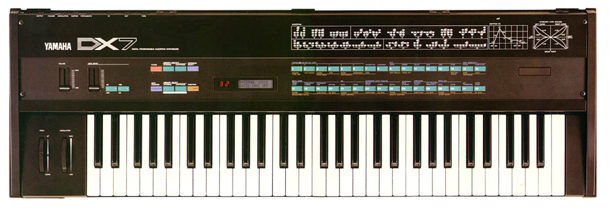
\includegraphics[width=0.95\textwidth]{dx7.png}
\caption{Yamaha DX7}
\label{fig:dx7}
Quelle: \url{http://www.electricdruid.net/images/interface/larger/YamahaDX7.jpg}
\\Stand 09.06.2015
\end{figure}

Durch den großen Erfolg des DX7 konnte Yamaha in den nachfolgenden Jahren viele Weiterentwicklungen auf den Markt bringen. In den Jahren 1983 bis 1989 brachte Yamaha über 20 weitere digitale Synthesizer heraus. Jedoch wurden über die Zeit andere Syntheseverfahren günstiger und für den Markt besser geeignet. Deshalb entwickelte Yamaha 1990 mit dem SY77 Synthesizer ein Gerät, das FM-Synthese und ein anderes digitales Klangsyntheseverfahren namens Sampling in Einem vereinte.\cite{fmGS1}

Ab Mitte der 1990er wurden Personal Computer leistungsfähig genug, um Synthesizer ohne Verzögerung durch eine Midi Tastatur ansprechbar zu machen. Heutzutage findet digitale Audioverarbeitung nahezu ausschließlich softwareseitig statt, weshalb Hardwaresynthesizer wie der DX7 an Bedeutung verloren haben. Speziell dieser wurde jedoch durch die Firma Native Instruments in Form des FM7 in Software nachgebaut. Dessen Weiterentwicklung namens FM8 findet heute noch Verwendung. Auch ist der DX7 heute bei Nostalgikern noch sehr beliebt.\cite{fmGS1}

\section{Technisches}

\subsection{Formel vorstellen \& Variablen klären}
\subsubsection{Auffrischung: Kosinusfunktion mit Parametern}
\subsubsection{Erklärung: Trägerfrequenz, Modulationsfrequenz, Modulationsindex}

\subsection{Besonderheiten der FM-Synthese}
\FloatBarrier
\subsubsection{Phasenmodulation als FM}
Frequenzmodulation (FM) und Phasenmodulation (PM) können unter dem Oberbegriff Winkelmodulation zusammen gefasst werden. Im Folgenden soll der Zusammenhang zwischen PM und FM genauer beschrieben werden. Zuerst wird die mathematische Herleitung der beiden Modulationen beschrieben. Anschließend wird die Ähnlichkeit der beiden Verfahren erörtert und im Kontext der Akustik beschrieben. Interessanterweise führte die Publikation von Chowning zu anfänglicher Verwirrung, da er in seinem Artikel eine Formel beschreibt, die einer PM gleicht und ein MUSIC V Patch der eine FM beschreibt. \cite{rossum1999method} Des Weiteren kann dem Yamaha Patent für die Implementierung eines FM-Synthesizer entnommen werden, dass Yamaha ihre FM-Synthese über eine PM erzeugte. \cite{oya1987electronic} 

Wie der Name Winkelmodulation andeutet, wird der Phasenwinkel eines Trägersignales in Abhängigkeit eines Modulationssignals verändert. Die Amplitude \(A\) bleibt während der Modulation konstant. In der allgemeinsten Form kann ein winkelmoduliertes Signal als Sinusfunktion eines sich zeitlich ändernden Winkels beschrieben werden:
\begin{equation}
s(t)=A*sin(\theta(t))
\label{eq:signal_basis_funktion}
\end{equation}
Dabei wird \(\theta(t)\) als \textit{momentaner Winkel} bezeichnet und ist als Summe der konstanten Kreisfrequenz $\omega_0$ multipliziert mit der Zeit $t$ und der \textit{momentanen Phase} $\varphi(t)$ definiert:
\begin{equation*}
\theta(t)=\omega_0t + \varphi(t)
\end{equation*}

Wird nun die momentane \textbf{Phase} des Trägersignals proportional zum Modulationssignal \(p(t)\) verändert, erhält man das \textbf{phasenmodulierte} Signal \(s_{PM}(t)\). \cite[S. 209]{lathi}
Für die momentane Phase ergibt sich folgende einfache Formel:
\begin{equation}
\varphi(t)=\varphi_0+k_{PM}*p(t)
\label{eq:varphi_t}
\end{equation}
Für akustische Anwendungen wird der konstante Teil \(\varphi_0\) der Phase nicht benötigt und wird als 0 angenommen. Bei \(k_{PM}\) handelt es sich um eine Proportionalitätskonstante, welche Modulatorkonstante genannt wird. Die Modulatorkonstante bestimmt, wie stark das Modulationssignal auf das Trägersignal einwirkt. Wird nun \(\theta(t)\) in die allgemeine Formel~\ref{eq:signal_basis_funktion} für ein moduliertes Signal substituiert und das obige \(\varphi(t)\) eingesetzt, ergibt sich die Formel für das phasenmodulierte Signal:
\begin{equation}
s_{PM}(t)=A*sin(\omega_0t + \varphi(t))=A*sin(\omega_0t+k_{PM}*p(t))
\label{eq:s_pm}
\end{equation}
Für die Herleitung der Frequenzmodulation muss zuvor noch der Begriff der \textit{momentan Kreisfrequenz} \(\omega_m(t)\) eingeführt werden.
Diese entspricht der Änderung des Phasenwinkels in Abhängigkeit der Zeit. Daher kann die momentan Kreisfrequenz durch die erste Ableitung des Phasenwinkels nach der Zeit $\dot \theta(t)$ bestimmt werden. \cite[S. 209]{lathi}
\begin{equation}
\omega_m(t)=\dot \theta(t)=\frac{d\theta(t)}{dt}=\frac{d[\omega_0t+\varphi(t)]}{dt}=\frac{d\omega_0t}{dt}+\frac{d\varphi(t)}{dt}=\omega_0+\frac{d\varphi(t)}{dt}
\label{eq:omega_m_herleitung}
\end{equation}
Wieso dieser Zusammenhang gültig ist, lässt sich einfach veranschaulichen. Bei \(\omega_m\) handelt es sich um die Kreisfrequenz, also wie häufig eine Schwingung einen Kreis pro Zeitspanne durchläuft, hier in Sekunden. Bei einer Kreisfrequenz von \(\omega=2 s^{-1}\) wird ein Phasenwinkel von \(4\pi\) pro Sekunde überstrichen. Wird nun die Kreisfrequenz erhöht, wird ein größerer Phasenwinkel überstrichen. Daher gibt die momentane Kreisfrequenz die Änderungsrate des momentanen Phasenwinkels zu einem bestimmten Zeitpunkt \(t\) an. Da die Änderung einer Funktion der Ableitung dieser Funktion entspricht, ergibt sich der Zusammenhang aus der obigen Formel. Eine Analogie aus der Physik hierzu ist der Zusammenhang zwischen Weg \(s(t)\) und Geschwindigkeit \(v(t)\). Die Geschwindigkeit gibt die Änderung des Weges pro Zeiteinheit vor und somit gilt, \(\dot{s(t)}=v(t)\). In unserem Zusammenhang verhält sich die Kreisfrequenz analog zur Geschwindigkeit und der Phasenwinkel ist im Prinzip die Strecke ausgedrückt als Winkel.

Wird die momentane \textbf{Frequenz} des Trägersignals proportional zum Modulationssignal \(f(t)\) verändert, erhält man das \textbf{frequenzmodulierte} Signal \(s_{FM}(t)\). \cite[S. 210]{lathi} Für die momentane Frequenz ergibt sich analog zur Phasenmodulation folgende Formel:
\begin{equation}
\omega_m(t)=\omega_0+k_{FM}*f(t)
\label{eq:omega_m}
\end{equation}

Bei \(k_{FM}\) handelt es sich wieder um eine Modulatorkonstante und gibt an wie stark das Modulationssignal das Trägersignal beeinflusst. Um nun das frequenzmodulierte Signal zu erhalten muss die momentan Frequenz, analog wie bei der Phasenmodulation, in \(s(t)\) eingesetzt werden. Jedoch kommt \(\omega_m\) nicht direkt in \(s(t)\) oder \(\theta(t)\) vor. Aus Formel~\ref{eq:omega_m_herleitung} ist bekannt, dass die momentane Frequenz gleich der ersten Ableitung des momentan Winkels \(\theta(t)\) ist. Im Umkehrschluss bedeutet das, dass die Integration von \(\omega_m\) nach der Zeit gleich \(\theta(t)\) sein muss.
\begin{equation*}
\theta(t)=\int_0^t{\omega_m(t)} dt = \int_0^t{\omega_0 + k_{FM}*f(t)} dt = \omega_0t + k_{FM} * \int_0^t{f(t)} dt
\end{equation*}
Setzt man diesen Term in \(s(t)\) ein, erhält man die Formel für ein frequenzmoduliertes Signal
\begin{equation}
s_{FM}(t)=A*sin(\omega_0t + k_{FM} * \int_0^t{f(t)} dt)
\label{eq:s_fm}
\end{equation}
Es sei angemerkt, dass wissentlich die Integrationskonstante mit Null gleichgesetzt wurde und somit nicht in den Formeln auftritt, da sie für unsere Beobachtungen unerheblich ist und die Terme nur unnötig verkomplizieren würde.

Wie einführlich erklärt, ist die Phasenmodulation mit der Frequenzmodulation verwandt. Wie ähnlich die beiden Verfahren sind, ist leicht ersichtlich an den Formeln für die modulierten Signalen~\ref{eq:s_pm} und \ref{eq:s_fm}. Beide Formeln sind bis auf die letzte Addition gleich. Daraus lässt sich eine Bedingung ableiten, welche beschreibt wann eine FM durch eine PM oder umgekehrt dargestellt werden kann. Dies ist genau dann möglich, wenn die Signale \(s_{PM}(t)\) und \(s_{FM}(t)\) gleich sind. Daraus ergibt sich für die Modulationssignale \(p(t)\) und \(f(t)\) folgende Beziehung:
\begin{equation}
k_{PM}*p(t)=k_{FM} * \int_0^t{f(t)} dt
\end{equation}

Vorausgesetzt \(k_{PM}\) ist gleich \(k_{FM}\), dann können beide Faktoren aus der Gleichung eliminiert werden. Ist es nun möglich, für \(f(t)\) eine Ableitung zu finden, kann eine PM durch eine FM dargestellt werden. Durch die Ableitung von \(\int{f(t)}\) wird das Integral aufgehoben und die Gleichung reduziert sich zu einem einfachen \(p(t)=f(t)\). Umgekehrt gilt, dass genau dann eine FM durch eine PM dargestellt werden kann, wenn \(p(t)\) integrierbar ist. Unter diesen Bedingungen sind beide Verfahren mathematisch betrachtet gleich. Daher kann nur anhand der Betrachtung eines modulierten Signals nicht darauf zurück geschlossen werden, ob es mit einer Phasen- oder Frequenzmodulation moduliert wurde. Die unterschiedlichen Namen (FM, PM) zeigen somit nur, welche Größe des Modulationssignals (\(f(t), p(t)\)) proportional ist. \cite[S. 210]{lathi}
Eine weitere, erwähnenswerte Eigenschaft lässt sich gewinnen, wenn der momentane Phasenwinkel beider Verfahren gegenüber gestellt wird. Während \(\varphi(t)\) für PM durch die Formel~\ref{eq:varphi_t} gegeben ist, muss \(\varphi(t)\) für FM durch gleichsetzten der Formeln~\ref{eq:omega_m_herleitung} und \ref{eq:omega_m} gewonnen werden:
\begin{eqnarray*}
\omega_0+\frac{d\varphi(t)}{dt}&=&\omega_0+k_{FM}*f(t) \\
\frac{d\varphi(t)}{dt}&=&k_{FM}*f(t)
\end{eqnarray*}
Draus ergibt sich für ein gemeinsames Modulationssignal \(m(t)\) folgender Zusammenhang:
\begin{center}
\fbox{\parbox{7.5cm} { 
	\begin{eqnarray*}
	\varphi(t)&=&k_{PM}*m(t) : \textbf{PM} \\
	\frac{d\varphi(t)}{dt}&=&k_{FM}*m(t) : \textbf{FM}
	\end{eqnarray*}
}}
\end{center}
Da \({d\varphi(t)}/{dt}\) die Ableitung und somit die Änderung von \(\varphi(t)\) ist, ändert sich \(\varphi(t)\) wenn die Ableitung sich ändert und umgekehrt. PM und FM treten also immer gleichzeitig auf.

Bisher wurde nur das modulierte Signal betrachtet und dessen Abhängigkeit von den allgemeinen Modulationssignalen \(p(t)\) bzw. \(f(t)\). Für die bisherigen Erkenntnisse war es einfach nicht notwendig, sich auf eine spezifische Modulationssignale festzulegen. Diese allgemeine Betrachtung ist jedoch mehr für die Nachrichtentechnik interessant als für einen FM-Synthesizer.
Daher werden die folgenden Formeln im Kontext der Akustik betrachtet und weniger streng mathematisch wie bisher. So kann zum Beispiel das menschliche Gehör keine initiale Phasenverschiebungen wahrnehmen. Dies erlaubt Umformungen von Termen, die mathematisch nicht korrekt sind, jedoch am Ergebnis, also dem hörbaren Klang, keine Auswirkung haben. Deshalb ist es auch korrekt, bei den obigen Umformungen den initialen Phasenwinkel $\varphi_0$ zu ignorieren. Des Weiteren wird im Folgenden ein sinusförmiges Signal als Modulator verwendet, welches sowohl für die PM als auch die FM verwendet wird und wie folgt definiert ist:
\begin{equation}
m(t)=f(t)=p(t)=sin(\omega_m t)
\end{equation}
Wobei \(\omega_m\) die Modulationskreisfrequenz darstellt. Eingesetzt in die Formeln für PM und FM ergibt sich
\begin{eqnarray*}
s_{PM}(t)&=&A*sin(\omega_0t+k_{PM}*sin(\omega_m t)) \\
s_{FM}(t)&=&A*sin(\omega_0t+k_{FM}*\int_0^t{sin(\omega_m t)} dt)
\end{eqnarray*}
Die von Chowning vorgestellte Formel gleicht der Formel für eine PM, \cite{chowningPaper} wobei Chowning seine Formel als Frequenzmodulation vorstellt. Wieso diese Aussage trotzdem korrekt ist, wird im Folgenden gezeigt. Im ersten Schritt muss das Integral innerhalb von \(s_{FM}\) ausgerechnet werden:
\begin{equation*}
s_{FM}(t)=A*sin(\omega_0t-\frac{k_{FM}}{\omega_m}*cos(\omega_m t))
\end{equation*}
Mathematisch gesehen, unterscheidet sich diese Formel zu einer Phasenmodulation. Genauer gesagt, ergibt sich durch die Integration eine Verschiebung von einer Phase, da ein negativer Kosinus genau eine Phase verschoben zu einem Sinus ist. Wie bereits erwähnt, nimmt das Gehör jedoch keine initiale Phasenverschiebungen wahr. Unter dieser Annahme, kann der negative Kosinus mit einem positiven Sinus ausgetauscht werden, ohne eine hörbare Veränderung des Tons zu erzeugen.
\begin{equation*}
e(t)=A*sin(\omega_0t+\frac{k_{FM}}{\omega_m}*sin(\omega_m t))
\end{equation*}
Die dadurch gewonnene Formel ähnelt in der Struktur der von Chowning vorgestellten Formel schon sehr. Jedoch ist in der obigen Formel der Modulationsindex $I$ nicht direkt ersichtlich. Dieser ist bei Chowning als $I=d/\beta$ definiert. Wobei $d$ dem Frequenzhub entspricht und $\beta$ der Modulationsfrequenz $\omega_m$ (s. Kapitel~\ref{chowningparameter}). Für den Frequenzhub $\Delta f$ gilt: \cite[S. 219]{lathi}
\begin{equation*}
\Delta f = k_{FM}*[\dot f(t)]_{\max}
\end{equation*}
Da unser $f(t)$ eine Sinusfunktion darstellt, entspricht die Ableitung $\dot f(t)$ einer Kosinusfunktion und somit ist ihr Maximum gleich $1$ und entfällt in der obigen Formel. Somit reduziert sich der Frequenzhub zu $\Delta f=k_{FM}$ und kann in die obige Formel eingesetzt werden. Dadurch kann nun $\Delta f / \omega_m$ durch den Modulationsindex $I$ substituiert werden und es ergibt sich die originale Formel nach Chowning:
\begin{equation}
e(t)=A*sin(\omega_0t+I*sin(\omega_m t))
\label{eq:FM_Chowning}
\end{equation}
Diese Formel entspricht somit der von Chowning vorgestellten Formel für eine FM-Synthese und ist im Kontext der Akustik korrekt.



\FloatBarrier
\subsubsection{Seitenfrequenzbänder (Evtl. Besselfunktion)}
\label{bulli:ohrToeneUndFrequenzen}
Ein Ton wird durch eine einfache Sinusschwingung erzeugt. Die Tonstärke, also die Lautstärke eines Tones, hängt von der Amplitude der Schwingung ab. Je größer die Amplitude desto lauter wirkt der Ton. Die Frequenz einer Schwingung empfindet der Mensch als Tonhöhe. Je größer die Frequenz der Schwingung desto höher wird der Ton empfunden. 
Das menschliche Ohr nimmt Frequenzen zwischen 16 Hz und 20 kHz wahr. Mit zunehmenden Alter nimmt die obere Hörschwelle ab. \cite[S. 199]{borucki}
Ein natürlicher Klang setzt sich nicht aus einer einzigen Frequenz zusammen, sondern aus mehreren Teiltönen. Jeder Teilton entspricht einem Sinuston mit einer bestimmten Frequenz, welche ein ganzzahliges Vielfaches des tiefsten Teiltones ist. Der tiefste Teilton, also der Teilton mit der niedrigsten Frequenz, wird als Grundton bezeichnet. \cite[S. 87]{borucki} 
Dabei kann das menschliche Gehör die Tonhöhe bestimmen, auch wenn der Grundton schwach ausgeprägt oder nicht vorhanden ist. \cite[S. 4]{zwicker} Abbildung~\ref{fig:geige} zeigt die Wellenform eines Geigentones und dem dazu gehörigen Frequenzspektrums. Obwohl der Grundton wenig dominiert, die ersten acht Frequenzen sind in etwa gleichstark, würde das Ohr die Tonhöhe richtig erkennen. Des Weiteren nehmen wir neben der Tonhöhe und Lautstärke eines Tones etwas Weiteres war. Das Spektrum eines Tones gibt uns ein Gefühl für unterschiedliche Klänge. Dieses Empfinden wird als Klangfarbe bezeichnet und lässt uns z.B. zwischen verschiedenen Instrumenten unterscheiden. \cite[S. 5]{zwicker} \cite[S. 226]{raichel}
Warum die Teiltöne entscheidend für den Klangcharakter sind, erkennt man an der stark vereinfachten Funktionsweise des menschlichen Ohres. Die Schallwellen eines Klangs versetzten im Ohr, genauer in der Gehörschnecke, eine Flüssigkeit in Schwingung. Dadurch, dass die Gehörschnecke sich verengt, treffen die unterschiedlichen Frequenzen in Kombination mit der Amplitude, an unterschiedlichen Stellen auf Sinneshaare, welche die entsprechenden elektrischen Signale an das Gehirn weiterleiten. \cite[S. 87 f.]{zwicker}

\begin{figure} [ht]
\centering
  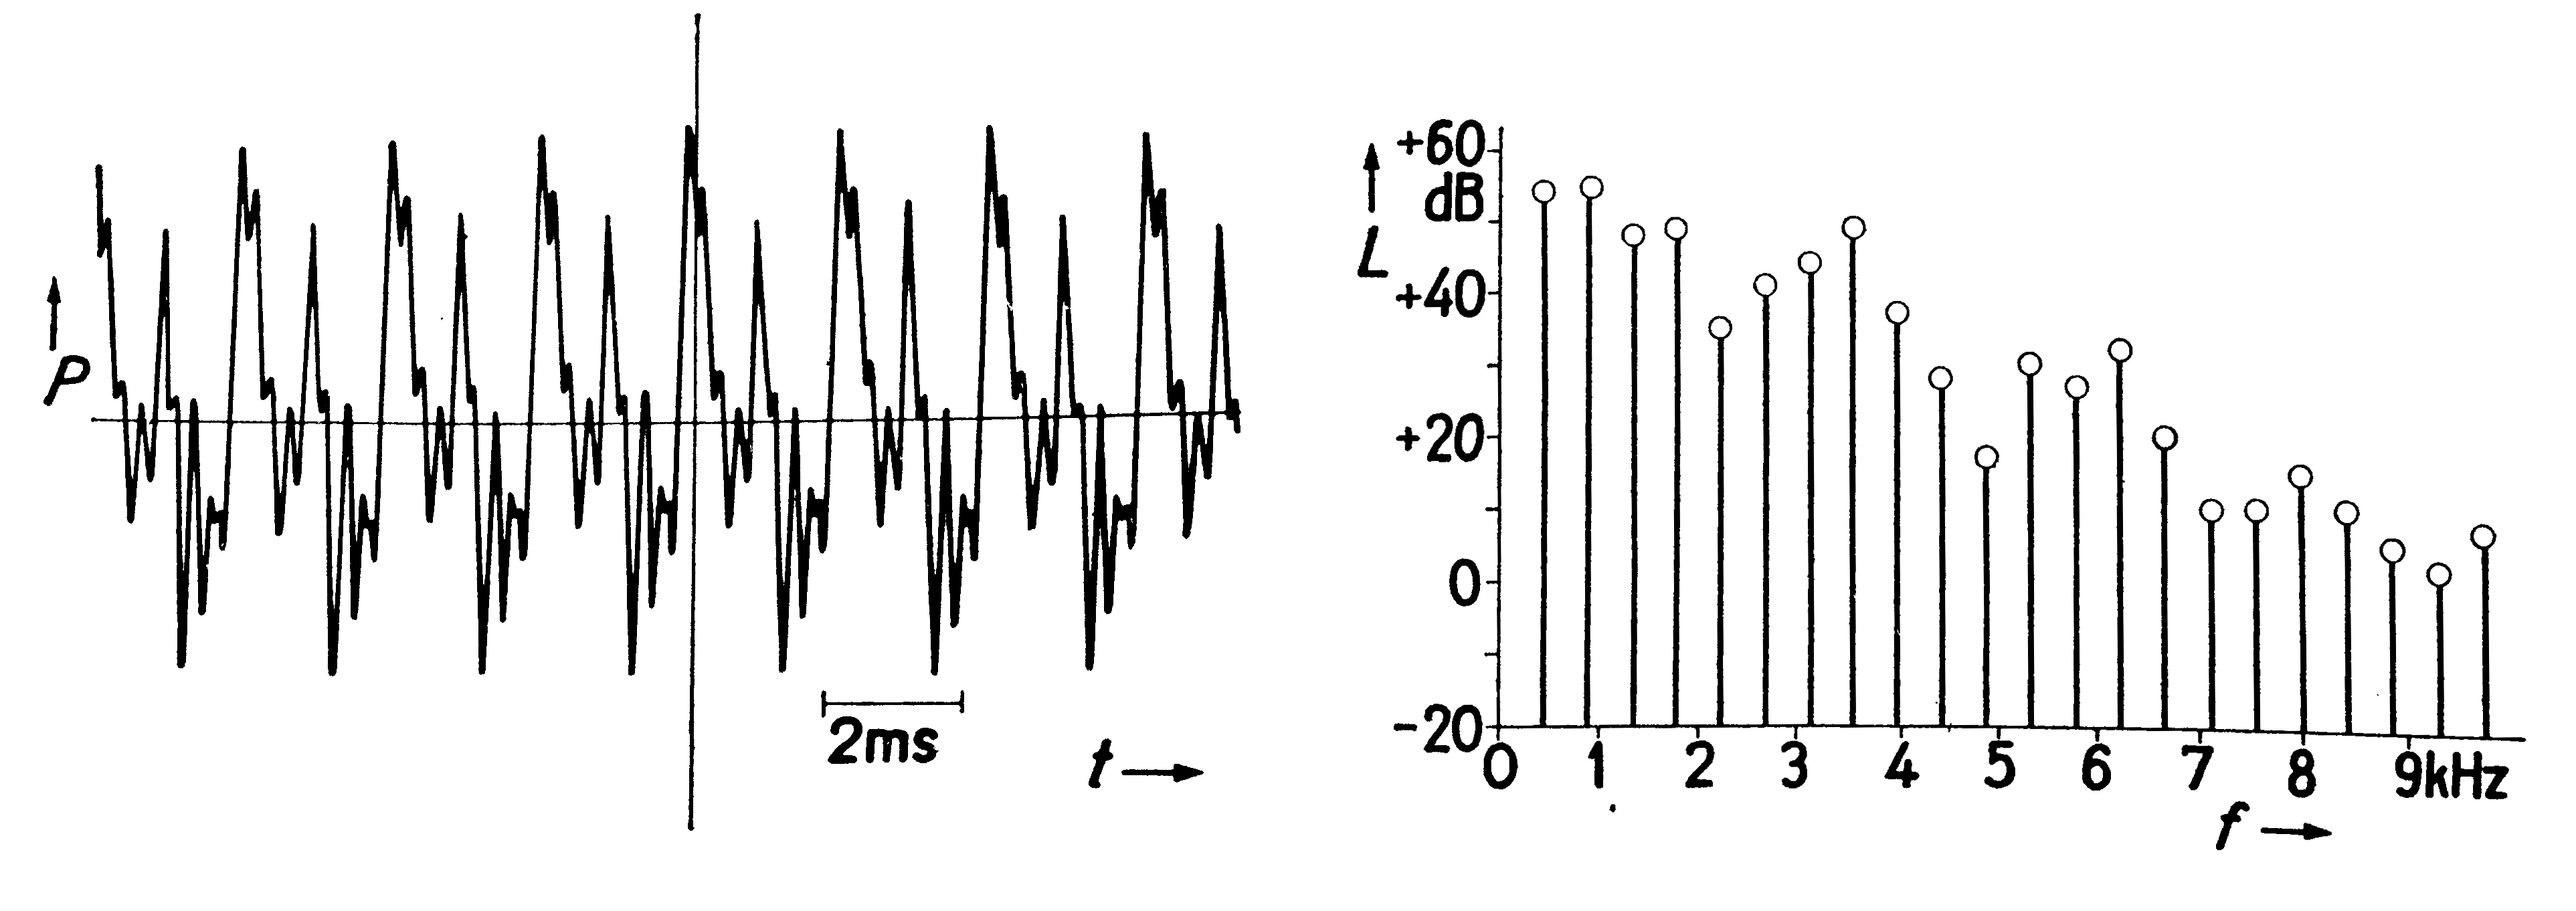
\includegraphics[width=0.95\textwidth]{GeigenTon.png}
\caption{Links: Schalldruck eines Geigenklangs; Rechts: Frequenzspektrum dieses Klanges}
\label{fig:geige}
Quelle: \cite[S. 4]{zwicker}
\end{figure}
\FloatBarrier

Um daher einen ungefähren Eindruck eines synthetisierten Tones zu bekommen, reicht es nicht aus, die berechnete Kurve (Wellenform) zu betrachten, welche eine Funktion der Zeit ist. Daher muss eine Alternative Darstellung des Signals gesucht werden. Ein \textbf{Frequenzspektrum} berechnet die Intensität einer gegeben Frequenz und ist somit eine Funktion der Frequenz. Das Frequenzspektrum lässt sich durch Fourier Analyse bestimmen. So kann jede komplexe Sinuswelle als Fourier Reihe dargestellt werden und somit als Addition aus mehreren Teilsinuswellen mit unterschiedlichen Amplituden. \cite[S. 33]{raichel} Durch mathematische Umformungen (siehe Kap.~\ref{matze:simplefm}), kann die Formel der FM-Synthese~\ref{eq:FM_Chowning} als folgende Summe dargestellt werden: \cite{chowningPaper}

\begin{equation}
\begin{split}
s(t)=A*\{\; & J_0(I)*\sin(\omega_c t)  \\
         +&J_1(I)*[\sin(t*(\omega_c + \;\,\omega_m))-\sin(t*(\omega_c-\;\,\omega_m))] \\
         +&J_2(I)*[\sin(t*(\omega_c + 2\omega_m))+\sin(t*(\omega_c-2\omega_m))] \\
         +&J_3(I)*[\sin(t*(\omega_c + 3\omega_m))-\sin(t*(\omega_c-3\omega_m))] \\
         +&....\}
\end{split}
\label{eq:chowningAddition}
\end{equation}

Hier bezieht sich $J_\nu(x)$ auf die Bessel Funktionen erster Ordnung, mit $\nu,x \in \mathbb{R}$. \cite[S. 223]{temme} Im Zusammenhang mit der FM-Synthese werden jedoch nur ganzzahlige $\nu$ Werte benötigt. Um diesen Umstand zu verdeutlichen wird im Folgenden $\nu$ als $n$ angegeben. Abbildung~\ref{fig:bessel2D} stellt die ersten drei Bessel Funktionen dar.

\begin{figure} [ht]
\centering
  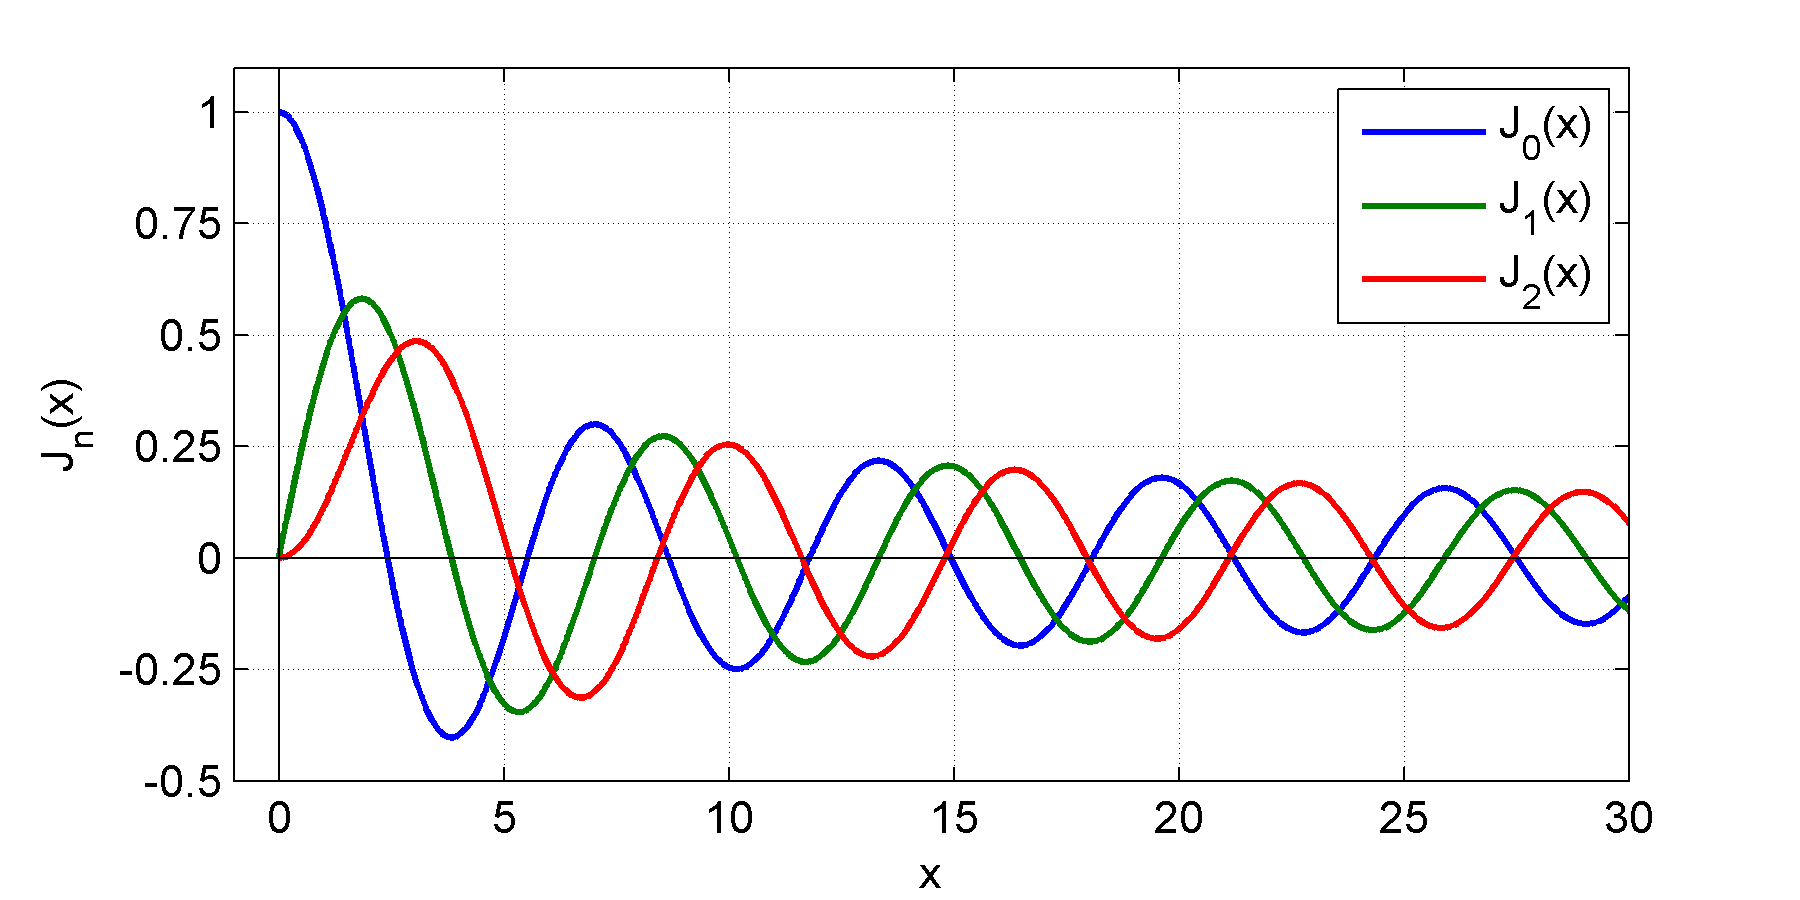
\includegraphics[width=0.80\textwidth]{Bessel2D.png}
\caption{2D-Plot der Bessel Funktionen $J_0$, $J_1$ und $J_2$.}
\label{fig:bessel2D}
Quelle: Eigene Darstellung mit MATLAB
\end{figure}

\FloatBarrier


Allgemein sind die Bessel Funktionen Lösungen für die Besselsche Differentialgleichung.\cite[S. 220]{temme} Bei der FM-Synthese treten sie in Erscheinung, sobald die Formel~\ref{eq:FM_Chowning} der FM-Synthese als Fourier-Reihe dargestellt wird. Eine Fourier-Reihe setzt sich aus der Addition aus Sinus Funktionen multipliziert mit einem Fourier-Koeffizienten zusammen. Für die FM-Synthese entspricht dieser Koeffizient der Bessel Funktionen erster Ordnung. \cite[S. 221]{lathi} Die genaue mathematische Herleitung soll an dieser Stelle nicht behandelt werden. Es soll jedoch angemerkt sein, dass $J_n(x)$ nicht elementar berechnet werden kann und numerisch bestimmt werden muss.\cite[S. 385]{abramowitz} Funktionswerte können in geeigneten Tabellen nachgeschlagen werden. \cite{davis}

Wie oben beschrieben, besteht ein Klang nicht nur aus seinem Grundton sondern auch aus Seitenfrequenzbänder. Theoretisch treten unendlich viele solcher Frequenzbänder auf, jedoch werden diese nicht mehr vom Ohr wahrgenommen, wenn sie eine gewisse Grenze an Intensität unterschreiten. Die Amplitude des Grundtones lässt sich durch $J_0(I)$ berechnen, wobei $I$ für den Modulationsindex steht. Dies lässt sich auch einfach aus Formel~\ref{eq:chowningAddition} entnehmen. Der erste Additionsterm $J_0(I)\sin(\omega_c t)$ entspricht der Trägerfrequenz. Bei einem Modulationsindex von $I=0$ findet keine Frequenzmodulation statt. An Abbildung~\ref{fig:bessel2D} wird ersichtlich, dass $J_0(0)=0$ ist. Für alle weiteren Bessel Funktionen gilt $J_n(0)=0$, damit reduziert sich die Addition aus Formel~ \ref{eq:chowningAddition} auf die Grundschwingung $1*sin(\omega_c t)$ und deckt sich somit mit unserer Erwartung, dass keine Modulation statt findet. Daraus lässt sich erschließen, dass die Trägerfrequenz $\omega_c$ dem Grundton entspricht. Die Amplitude der n-ten Seitenschwingung berechnet sich durch $J_n(I)$ wobei $n$ für die erste, zweite, dritte usw. Seitenfrequenz steht. Für Oberschwingungen ist $n$ immer positiv, für Unterschwingungen negativ. Bei negativen $n$ Werten gilt folgender Zusammenhang: \cite[S. 223]{temme}
\begin{equation*}
J_{-n}(x)=(-1)^nJ_n(x)
\end{equation*}

Die Formel drückt aus, dass für ungerade Seitenschwingungen das Vorzeichen invertiert werden muss und bei geraden Seitenschwingungen nicht. Dies ist auch in der Summenformel~\ref{eq:chowningAddition} ersichtlich. Für ungerade $n$ Werte werden die Sinus Werte subtrahiert, bei geraden $n$ addiert. Dies wird nicht offensichtlicher, wenn $J_n(I)$ mit der Klammer multipliziert wird, wie in Formel~\ref{eq:FormelinchenBessel} in Kapitel~\ref{matze:simplefm}.

\label{bulli:besselModIndexZusammenahang}
Wird nun der Modulationsindex stetig erhöht, wird Energie aus der Grundfrequenz genommen und auf die Seitenbänder verteilt. Dies lässt sich wieder an Abbildung~\ref{fig:bessel2D} erkennen. Wird $I$ größer, fällt die Amplitude von $J_0(I)$ ab und die restlichen Bessel Funktionen steigen an. $J_0(I)$ durchläuft den Nullpunkt bei $\approx2,5$, das bedeutet bei einem Modulationsindex von ungefähr $2,5$ ist der Grundton nicht im Frequenzspektrum vorhanden, sondern nur noch Seitenfrequenzen. In Abbildung~ \ref{fig:chowningEnergieVerteilung} wird der Modulationsindex von $0$ bis $4$ inkrementiert. Es wird ersichtlich, wie immer mehr Seitenfrequenzen entstehen und dabei die Grundfrequenz abnimmt. In Abbildung~ \ref{fig:chowningEnergieVerteilung} wird der Betrag der Amplitude dargestellt, somit wird die Grundfrequenz für $I=3$ im Vergleich zu $I=2$ wieder größer, da die Bessel Funktion den Nullpunkt durchlaufen hat und im negativen Bereich größer wird, bis das lokale Minimum erreicht wird und der Betrag wieder bis $0$ abnimmt.

\begin{figure} [ht]
\centering
  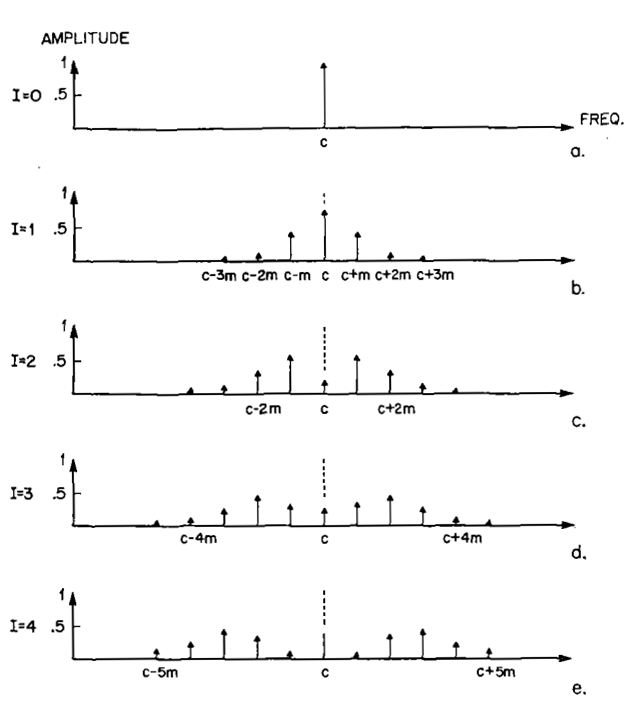
\includegraphics[width=0.5\textwidth]{Chowning_EnergieVerteilung.png}
\caption{Beispiel zur Veranschaulichung der zunehmender Bandbreite in Abhängigkeit eines wachsenden Modulationsindex. $c$ entspricht der Trägerfrequenz; $c\pm n*m$ entspricht der n-ten Seitenfrequenz.}
\label{fig:chowningEnergieVerteilung}
Quelle: \cite{chowningPaper}
\end{figure}
\FloatBarrier

An Abbildung~\ref{fig:chowningEnergieVerteilung} erkennt man auch, dass die Seitenfrequenzen sich symmetrisch in negativer und positiver Richtung zur Grundfrequenz ausbreiten. Dies erkennt man auch an Formel~\ref{eq:chowningAddition}, der innere Teil vom Sinus entspricht der Seitenfrequenz, wobei $(\omega_c+n*\omega_m)$ der n-ten Oberschwinung entspricht und $(\omega_c-n*\omega_m)$ der n-ten Unterschwinung. $J_n(I)$ gibt die Amplitude der n-ten Unter- und Oberschwinung an. 
Dies ist ein Vorteil der FM-Synthese im Vergleich zu anderen Sound Synthese Verfahren. Durch eine relativ simple Änderung des Modulationsindex können komplexe Klänge mit reichen Klangspektrum erzeugt werden.
Wie in Kapitel \nameref{PrinzipFM} beschrieben, ist es jedoch schwer das Ergebnis der FM-Synthese vorher zusehen. Dies liegt zum einen an dem schwingenden Verlauf der Bessel Funktionen und deren Zusammenspiel. TODO 'die 3D Darstellung der Besselfunktion kann diesen Faktor etwas abschwächen, da man durch die Darstellung ein Gefühl für die Funktion bekommt'

Zum Anderen an zwei Effekten bei der Bestimmung des Frequenzspektrums, die in Abbildung~ \ref{fig:chowningEnergieVerteilung} ignoriert wurden, machen die Vorhersehbarkeit noch schwerer. Der erste Effekt betrifft negative Seitenfrequenzen. Deren Vorzeichen invertiert wird und somit, anschaulich, an der Ordinate in den positiven Frequenzbereich reflektiert werden. [TODO warum ist das so?] Der zweite Effekt betrifft Frequenzen, die den selben Wert haben. Dabei werden die Amplituden der gleichen Frequenzen algebraisch addiert. Dies kann auch zuvor reflektierte Frequenzen betreffen. Daher kann es unter Umständen schwer sein, einen gegeben Klang durch FM-Synthese zu rekonstruieren, da man keine direkte Kontrolle über die Teiltöne wie bei der additiven Synthese hat. Abbildung~\ref{fig:chowningFreqReflektion} veranschaulicht das Verhalten der Seitenfrequenzen. Als einfaches Beispiel wählte Chowning $\omega_c=\omega_m=100$ und $I=4$.


\begin{figure} [ht]
\centering
  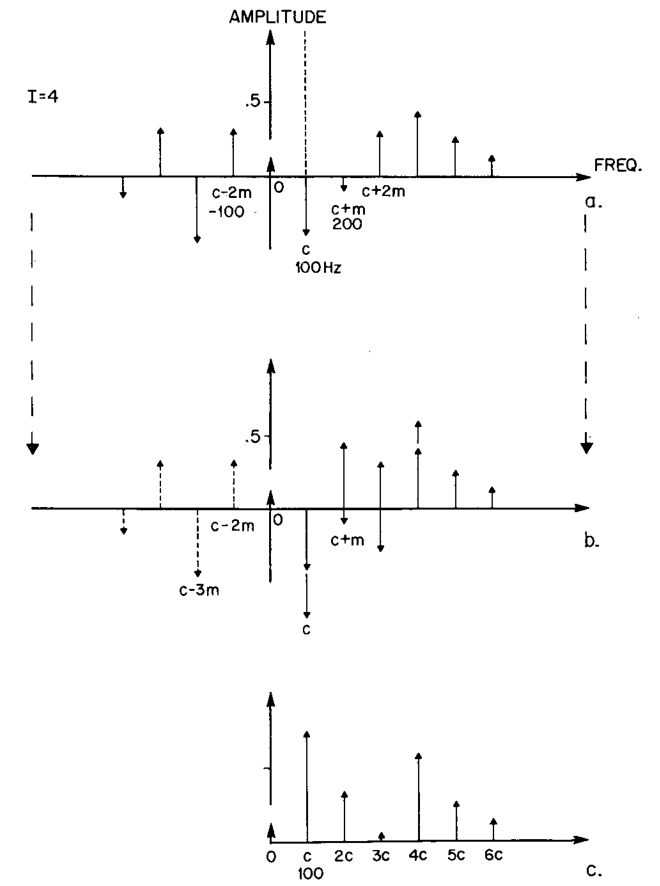
\includegraphics[width=0.5\textwidth]{ChowningFreqReflektion.png}
\caption{TODO}
\label{fig:chowningFreqReflektion}
Quelle: \cite{chowningPaper}
\end{figure}
\FloatBarrier





\begin{figure} [ht]
\centering
  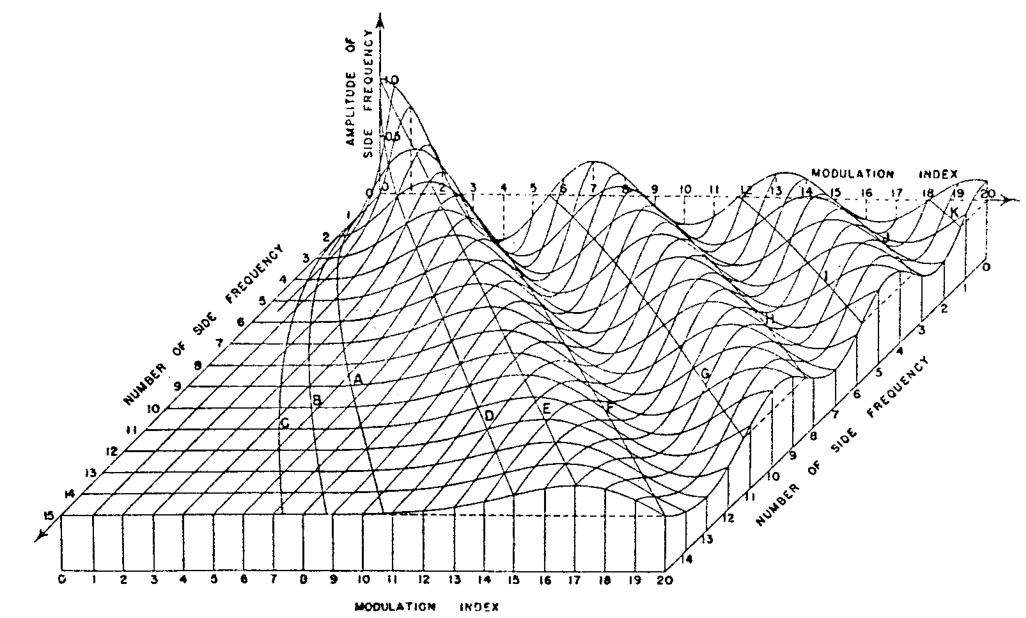
\includegraphics[width=0.95\textwidth]{ChowningBessel.png}
\caption{Besselfunktion $J_0$ bis $J_{15}$ und Modulationsindex $I$ von 0 bis 20. }
\label{fig:bessel3D}
Quelle: \cite{chowningPaper}
\end{figure}



Durch die zeitliche Änderung der Frequenz bei der Frequenzmodulation entstehen Seitenfrequenzbänder.


Das Frequenzspektrum eines natürlichen Tons ist selten statisch sondern variiert mit der Zeit. Diese Änderung der Teiltöne lässt das menschliche Ohr Töne unterschiedlich wahrnehmen. Durch die FM-Synthese lassen sich, im Vergleich zu anderen Syntheseverfahren, auf einfachen Weg komplexe und vielfältige Frequenzspektren künstlich erzeugen.

\FloatBarrier
\subsubsection{Harmonische Frequenzverhältnisse(Inkl. Vibrato)}
Bisher wurde nur wenig auf die beiden Frequenzparameter eingegangen. Diese können theoretisch beliebige Werte annehmen, so lange sie innerhalb des hörbaren Frequenzbereichs liegen. Ist das Ziel jedoch harmonische Klänge für Musik zu synthetisieren, müssen Trägerfrequenz und Modulationsfrequenz in einem besonderem Verhältnis stehen. Genauer gesagt muss das Verhältnis durch eine rationale Zahl beschrieben werden können, also durch einen Bruch aus zwei ganzen Zahlen $N_1$ und $N_2$. Somit gilt:
\begin{equation*}
\frac{f_c}{f_m}=\frac{N_1}{N_2}
\end{equation*}
Ist der Bruch $N_1/N_2$ zusätzlich gekürzt, ergibt sich für die Grundfrequenz $f_0$ der modulierten Schwingung folgende Gleichung:
\begin{equation*}
f_0=\frac{\omega_c}{N_1}=\frac{\omega_m}{N_2}
\end{equation*}
Für die Positionen der Seitenfrequenzen in der harmonischen Reihe des Klangs gilt:
% TODO formatierung
\begin{equation*}
k=N_1+n*N_2 \mbox{fuer} n=...,-2,-,1,0,1,2,...
\end{equation*}
Wobei $k$ die Nummer der Harmonischen entspricht und $n$ der n-ten Seitenfrequenz. Unter den obigen Bedingungen lassen sich weitere, für die Klangerzeugung hilfreiche, Aussagen treffen: \cite{chowningPaper}
\begin{lstlisting}[mathescape]
1) Die Trägerfrequenz ist immer die $N_1$-te Harmonische.
2) Für $N_2=1$ enthält das Spektrum alle Harmonischen und der Grundton entspricht der Trägerfrequenz.
3) Wenn $N_2$ gerade ist, enthält das Spektrum nur ungerade Harmonische.
4) Ist $N_2=3$, fehlt jede dritte Harmonische in der Reihe der Harmonischen.
\end{lstlisting}
Die Anzahl der Harmonische im modulierten Signal mit ausreichend großer Amplitude ist abhängig vom Modulationsindex. Für kleine Indizes und Frequenzverhältnisse mit $N_1\neq1$ kann der Grundton nicht im erzeugten Klang vorhanden sein. Die Seitenschwinungen im negativen Frequenzbereich, werden wie weiter oben beschrieben, an dem Ursprung ins Positive gespiegelt. Solang das Verhältnis eine rationale Zahl ist, werden diese Frequenzen genau auf die positiven Frequenzen der Harmonischen reflektiert und auf diese addiert.
Es entstehen somit keine neue Frequenzen neben den Harmonischen. Ist das Verhältnisse der beiden Frequenzen jedoch irrational, 
zum Beispiel $f_c/f_m=1/\sqrt{2}$, treffen die reflektierten Frequenzen nicht genau auf die positiven Frequenzen und erzeugen somit Seitenfrequenzen die kein ganzzahlig Vielfaches der Grundfrequenz sind. Es resultiert ein disharmonisches Klangspektrum.

Wie in \nameref{geschichteFMSynthese} beschrieben, entdeckte Chowning nach eigener Angabe die FM-Synthese beim Experimentieren mit einem Vibrato. Der Begriff Vibrato kommt aus der Musik und beschreibt eine oszillierende leichte Variation der Tonhöhe und somit der Frequenz. Dieser Effekt ist gerade bei Violinisten erwünscht und lässt den Ton "'reicher"' und "'zarter"' klingen. \cite[S. 422]{tobias} Da der Vibrato eine Abweichung der Tonhöhe und somit eine periodische Änderung der Frequenz ist, lässt sich einfach nachvollziehen wie Chowning beim Experimentieren mit verschiedenen Zahlwerten die FM-Synthese entdeckte. Von einem Vibrato wird gesprochen, wenn die Modulataionsfrequenz unter 20 Hz liegt.

TODO Vibrator Spektorgram













\FloatBarrier 

\subsection{Prinzipien der komplexen Frequenzmodulation}

Die bisherige Darstellung der Soundsynthese durch Frequenzmodulation (FM) hat sich auf die \textit{einfache} FM konzentriert, d.h. auf die Modulation eines einzigen Trägers durch einen einzelnen Modulator. Dadurch konnten die Prinzipien der Einflussnahme auf die Sounderzeugung über die Parameter von Trägerfrequenz, Modulationsfrequenz sowie den Modulationsindex analytisch klar isoliert werden. In der Praxis ist diese Limitation nicht notwendig, so dass zur Erzeugung komplexer Klangspektren auf den gleichzeitigen Einsatz mehrerer Träger und Modulatoren zurückgegriffen wird. Diese können dabei flexibel miteinander verschaltet werden. Man spricht in diesem Zusammenhang von der \textit{komplexen} FM. Im folgenden werden die Prinzipien der komplexen FM näher beleuchtet. Auch hier wird zunächst mit einer künstlichen Limitation gearbeitet und der bisher betrachtete Fall entweder um einen weiteren Träger erweitert oder um einen weiteren Modulator. Denkbar sind unter diesen Bedingungen zwei grundsätzliche Verschaltungsmuster, und zwar zum einen eine Parallelschaltung, zum anderen eine Reihenschaltung. Anschließend wird am Beispiel des digitalen Synthesizers \textit{FM 8} des deutschen Herstellers \textit{Native Instruments} beispielhaft gezeigt, inwiefern moderne Software die Klangerzeugung durch komplexe FM für den Benutzer handhabbar macht. 

\subsubsection{Parallelschaltung}

\paragraph{Parallele Träger mit jeweils eigenem unabhängigen Modulator 0,5 S}$\;$

Zur Vollständigkeit soll die simpelste Erweiterung der einfachen FM nicht unerwähnt bleiben, und zwar die Situation zweier paralleler Träger, denen je ein eigener Modulator zugeordnet ist (Abb 1). Dabei handelt es sich streng genommen noch um keine komplexe FM, da die Signalpfade beider Träger erst auf der Ebene des Gesamtausgangssignals gemischt werden und sich ansonsten nicht weiter beeinflussen. Jedes Träger-Modulator-Paar, also T1 mit M1 sowie T2 mit M2, folgt für sich genommen den Prinzipien der einfachen FM, so dass für jedes Paar die Lage der Seitenfrequenzbänder gesondert bestimmt und addiert werden kann. Lage und Amplitude der Seitenfrequenzbänder folgen direkt aus der gewählten Funktion für die Frequenzmodulation, auch wenn die Herleitung nichttrivial ist und Kenntnis der Eigenschaften der sogenannten \textit{Besselfunktion} voraussetzt. Alle Spektren und Wellenformen in Kapitel 3 dieser Seminararbeit wurden auf Basis folgender Funktion für die FM modelliert:
\begin{equation}\label{eq:SimpleFM}
f_{FM}(t) = \sin(w_ct + I\sin(w_mt)) \quad \text{mit} \quad w_ct \quad \text{als Träger-} \quad \text{und} \quad w_mt \quad \text{als Modulationsfreq.}
\end{equation}
Expandiert man diese über das trigonometrische Additionstheorem \begin{math} \sin(a + b) = \sin(a)\cos(b)+\cos(a)\sin(b) \end{math}, so erhält man 
\begin{equation}\label{eq:BesselZwischenform}
\sin(w_ct + I\sin(w_mt)) = \sin(w_ct)\cos(I\sin(w_mt)) + \cos(w_ct)\sin(I\sin(w_mt))
\end{equation}
Die inneren Terme \begin{math} \cos(I\sin(w_mt)) \end{math} und \begin{math} \sin(I\sin(w_mt)) \end{math} können über die erzeugende Funktion der Besselfunktion wie folgt ausgedrückt werden (der Beweis findet sich hier KREH):
\begin{equation}\label{eq:Besselsin}
\sin(I\sin(w_mt)) = 2J_1(I)\sin(w_mt)+2J_3(I)\sin(3w_mt)+...+2J_{2n+1}(I)\sin((2n+1)w_mt)+...
\end{equation}
\begin{equation}\label{eq:Besselcos}
\cos(I\sin(w_mt)) = J_0(I)+2J_2(I)\cos(2w_mt)+...+2J_{2n}(I)\cos(2nw_mt)+...
\end{equation}
Eingesetzt in \ref{eq:BesselZwischenform} können alle auftretende Terme der Form \begin{math} \sin(w_ct)\cos(2nw_mt) \end{math} über das Additionstheorem \begin{math} \sin(a)\cos(b) = \frac{1}{2}\left(\sin(x+y)+\sin(x-y)\right) \end{math} sowie alle Terme \begin{math} \cos(w_ct)\sin((2n+1)w_mt) \end{math} über  \begin{math} \cos(a)\sin(b) = \frac{1}{2}\left(\sin(x+y)-\sin(x-y)\right) \end{math} expandiert werden, so dass letztlich gilt (CHOW2): 
\begin{equation}
\begin{split}
\sin(w_ct + I\sin(w_mt)) \\ &\quad = J_0(I)\sin(w_ct) \\ &\quad + J_1(I)\left(\sin(w_ct + w_mt) - \sin(w_ct - w_mt)\right) \\ &\quad + J_2(I)\left(\sin(w_ct + 2w_mt)+\sin(w_ct-2w_mt)\right) \\ &\quad  + J_3(I)\left(\sin(w_ct + 3w_mt) - \sin(w_ct - 3w_mt)\right) \\ &\quad  + ...
\end{split}
\end{equation}
Dies kann übersichtlich zusammengefasst werden zu (KREH)
\begin{equation}
\sin(w_ct + I\sin(w_mt)) = \sum_{n=-\infty}^{\infty}J_n(I)\sin(w_ct+nw_mt)
\end{equation}
Das Frequenzspektrum für die einfache FM weist nun an der Frequenz \begin{math} w_c \end{math} sowie im positiven Bereich als auch im negativen Bereich stets im Abstand \begin{math} w_m \end{math} Seitenbänder mit einer Amplitude auf, wie sie die Besselfunktion als Koeffizient des entsprechenden Terms zurückliefert. Der Verlauf der Besselfunktion gibt dabei ab einem Modulationsindex größer ca. 2,5 auch negative Vorzeichen für die Seitenfrequenzen (ABB CHOW). Die für beide Träger-Modulatorenpaare nach obiger Formel jeweils ermittelten Frequenzspektren können in einem abschließenden Schritt einfach aufaddiert werden und bilden in Summe das Frequenzspektrum dieser Form der Parallelschaltung. Dies lässt sich in Matlab komfortabel visualisieren. Zunächst das erste Paar T1 und M1 (220:440,1):

Nun das zweite Paar T2 und M2 (230:500,1):

Bei beiden einfachen FM sieht man sehr gut, dass sich die Seitenfrequenzbänder in Abständen der Modulationsfrequenz um die Trägerfrequenz nach beiden Seiten ausbreiten. Und schließlich in der Parallelschaltung. Man sieht sehr gut, dass sich die Einzelspektren aufaddieren. 


\paragraph{Parallele Träger mit einem gemeinsamen Modulator}$\;$

Teilen sich zwei Träger T1 und T2 denselben Modulator M, kann das Frequenzspektrum ebenfalls als Summe zweier unabhängiger einfacher FM betrachtet werden. Hierzu kann einfach das Frequenzspektrum des einen Trägers T1 mit der Frequenz und dem Modulationsindex des Modulators M berechnet werden. Anschließend berechnet man das Frequenzspektrum für den zweiten Träger T2, wobei wieder Frequenz und Modulationsindex vom einzigen Modulator M bezogen werden. Aufsummiert ergibt sich dann das Gesamtspektrum. Das Interessante an dieser Form der Parallelschaltung  besteht in der Möglichkeit, für mehrere evtl. vorhandene Träger, deren Modulatoren dieselbe Modulationsfrequenz aufweisen, nur einen einzigen Modulator zu verwenden. Dadurch können diese anderen Modulatoren für andere Zwecke verwendet werden, z.B. um einen der Träger durch zwei Modulatoren zu modulieren (siehe das nächste Kapitel) oder sogar zum Modulieren des bereits eingesetzten Modulators (was dann der Kaskadenschaltung entspräche, siehe das übernächste Kapitel). Die Möglichkeit, denselben Modulator für verschiedene Träger zu verwenden bedeutet jedoch, dass die individuelle Modulierbarkeit beider Träger aufgegeben wird, da sich Änderungen an den Einstellungen von M zwangsläufig sowohl auf T1 als auch auf T2 auswirken. Die gleiche Mächtigkeit zweier paralleler Träger mit demselben Modulator im Vergleich zum Setup mit mehreren Trägern, die jeweils ihren eigenen Modulator, jedoch mit gleicher Frequenz und gleichem Modulationsindex, sei im Folgenden illustriert. Hier sehen wir das Spektrum zweier Träger, die jeweils von eigenen Modulatoren moduliert werden (220:440,3); (370:440,3):

Zum Vergleich Wellenform und Frequenzspektrum für zwei Träger (220 und 370), die sich denselben Modulator teilen (440, 3):

\paragraph{Einzelner Träger mit parallel geschaltetem Modulatorenpaar 1 S}$\;$

Wird ein einzelner Träger T von zwei parallel geschalteten Modulatoren M1 und M2 moduliert, kann das erzeugte Frequenzspektrum nicht mehr einfach als Summe der Spektren zweier einfacher FM begriffen werden, da sich die Auswirkungen der beiden Modulatoren auf den Träger gegenseitig beeinflussen und zahlreiche \textit{Kombinationsseitenfrequenzen} (CHOWNING)oder \textit{Intermodulationsfrequenzen]} (SCHOTTSTAEDT) entstehen. Das ist bereits aus der Formel für diese Spielart des FM direkt ersichtlich, die analog zu \ref{eq:SimpleFM} wie folgt lautet:
\begin{equation}
f_{FMmodpar}(t) = \sin(w_ct + I_1\sin(w_{m1}t) + I\sin(w_{m2}t))
\end{equation}
Nach mehrmaliger Anwendung der trigonometrischen Additionstheoreme zeigt sich bereits, dass diese Formel eine Vielzahl zusätzlicher Terme mit sich bringt:
\begin{equation}
\begin{split}
\sin(w_ct + I_1\sin(w_{m1}t) + I\sin(w_{m2}t)) \\ &\quad = \sin(w_ct)\cos(I_1\sin(w_{m1}t))\cos(I\sin(w_{m2}t)) \\ &\quad + \cos(w_ct)\sin(I_1\sin(w_{m1}t))\cos(I\sin(w_{m2}t)) \\ &\quad +\cos(w_ct)\cos(I_1\sin(w_{m1}t))\sin(I\sin(w_{m2}t)) \\ &\quad -\sin(w_ct)\sin(I_1\sin(w_{m1}t))\sin(I\sin(w_{m2}t))
\end{split}
\end{equation}
Substituiert man hier mit \ref{eq:Besselsin} und \ref{eq:Besselcos}, und wendet erneut die Additionstheoreme an, so ergibt sich übersichtlich:
\begin{equation}
\sin(w_ct + I_1\sin(w_{m1}t) + I\sin(w_{m2}t)) = \sum_{i=-\infty}^{\infty}\sum_{k=-\infty}^{\infty}J_i(I_1)J_k(I_2)\sin(w_ct + iw_{m1}t + kw_{m2}t)
\end{equation}



\subsubsection{Kaskadenschaltung}

\paragraph{Einzelner Träger mit in Reihe geschaltetem Modulatorenpaar 2 S}

\subsubsection{Komplexe Soundsynthese mit Native Instruments' \textit{FM8}}

\paragraph{Die FM-Matrix 1,5 S}


\paragraph{ADSR-Hüllkurven-Generator 0,5 S}

\section{Praktische Anwendung der FM-Synthese}
\FloatBarrier
\subsection{Nachbildung eines Instruments}
Bei der FM Synthese fällt es schwer vorauszusagen, was für ein Spektrum durch die Synthese erzeugt wird, dadurch ist es ein schwieriges Unterfangen mit dieser Technik ein echt wirkendes Instrument nachzubilden. Weitere Informationen hierzu in \ref{PrinzipFM} - \nameref{PrinzipFM}.
Trotzdem gibt es einige Methoden den generierten Klang natürlicher wirken zu lassen. Diese werden im weiteren Verlauf diese Kapitels vorgestellt und anschließend versucht den Klang eines Tones einer Querflöte nachzubilden.

\FloatBarrier
\subsubsection{Methoden zur Generierung eines Instrumententones mittels FM-Synthese}

Bei der Synthese eines Tones mittels FM-Synthese müssen zunächst die Parameter der FM-Synthese Formel festgelegt werden. Hierzu kann ein Frequenzspektrum des nachzubildenden Tones verwendet werden. Ausführliche Erklärung der einzelnen Parameter zu finden in Kapitel \ref{einfacheFM} - \nameref{einfacheFM}. Die Frequenz des größten Ausschlags im Spektrum (auch Grundfrequenz genannt) kann als Trägerfrequenz verwendet werden. Der Abstand der Grundfrequenz zur ersten Seitenfrequenz findet als Modulationsfrequenz Verwendung. Für den Modulationsindex kann nur eine grobe Schätzung vorgenommen werden, hierzu ist die Faustformel Modulationsindex + 2 = Anzahl der sichtbaren Seitenfrequenzen nützlich. Sollte mittels der normalen FM-Synthese kein zufriedenstellendes Ergebnis erzielt werden können, sollte mit der Komplexen FM-Synthese experimentiert werden. 

Bei der Komplexen FM-Synthese finden mehrere Träger oder mehrere Modulatoren Verwendung. Diese können in reihe oder parallel geschaltet werden. Außerdem kann auch die so genannte Feedback Frequenz Modulation genutzt werden, welche das voran gegangene Signal moduliert. \cite[S. 399 f.]{hornerPaper} Feedback FM wird vor allem eingesetzt um Rauschen zu erzeugen. Sie kann aber auch ein sehr komplexes Spektrum mit vielen Seitenfrequenzen erzeugen. Komplexe FM-Synthese findet Einsatz wenn die normale FM-Synthese nicht ausreichend komplexe Spektren erzeugt. Dies kann zum Beispiel der Fall sein wenn mehrere stetig fallende Seitenfrequenzen erzeugt werden sollen. Wenn bei einfacher FM-Synthese der Modulationsindex erhöht wird um mehr Seitenfrequenzen zu erzeugen, nimmt die Stärke der Grundfrequenz - definiert durch die Bessel Funktion - immer weiter ab und verteilt sich auf die Seitenfrequenzen - nachzulesen im Kapitel \ref{bulli:besselModIndexZusammenahang} - \nameref{bulli:besselModIndexZusammenahang}. Um dies zu vermeiden können die Modulatoren verschachtelt werden - nachzulesen im Kapitel \ref{Kaskadenschaltung} - \nameref{Kaskadenschaltung}

Eines der wichtigsten Grundbestandteile eines jeden Instrumententones ist die so genannte ADSR-Hüllkurve. Die Hüllkurve wird genutzt um die Amplitude des künstlich erzeugten Signals über den zeitlichen Verlauf festzulegen. ADSR steht für die einzelnen Phasen eines Tones: Attack, Decay, Sustain und Release. Diese Phasen sollen hier vereinfacht erklärt werden. Beim Drücken einer Taste wird der Ton angeschlagen und die Lautstärke des Tones steigt schnell bis zu einem maximal Wert an. Diese Phase wird Attack-Phase genannt. Nachdem die maximale Lautstärke erreicht wurde, startet die Decay Phase. In dieser Phase sinkt die Lautstärke schnell auf einen geringeren Wert ab. Danach befindet sich der Ton in der Sustain Phase und die Lautstärke bleibt gleich, solange der Ton gespielt wird. Sobald die Taste losgelassen wird, nimmt die Lautstärke wieder bis zu ihrem minimal Wert ab. In Abbildung \ref{fig:adsrDefault} ist der Verlauf der Lautstärke einer Standard ADSR-Hüllkurve noch einmal grafisch dargestellt.

\begin{figure} [ht]
\centering
  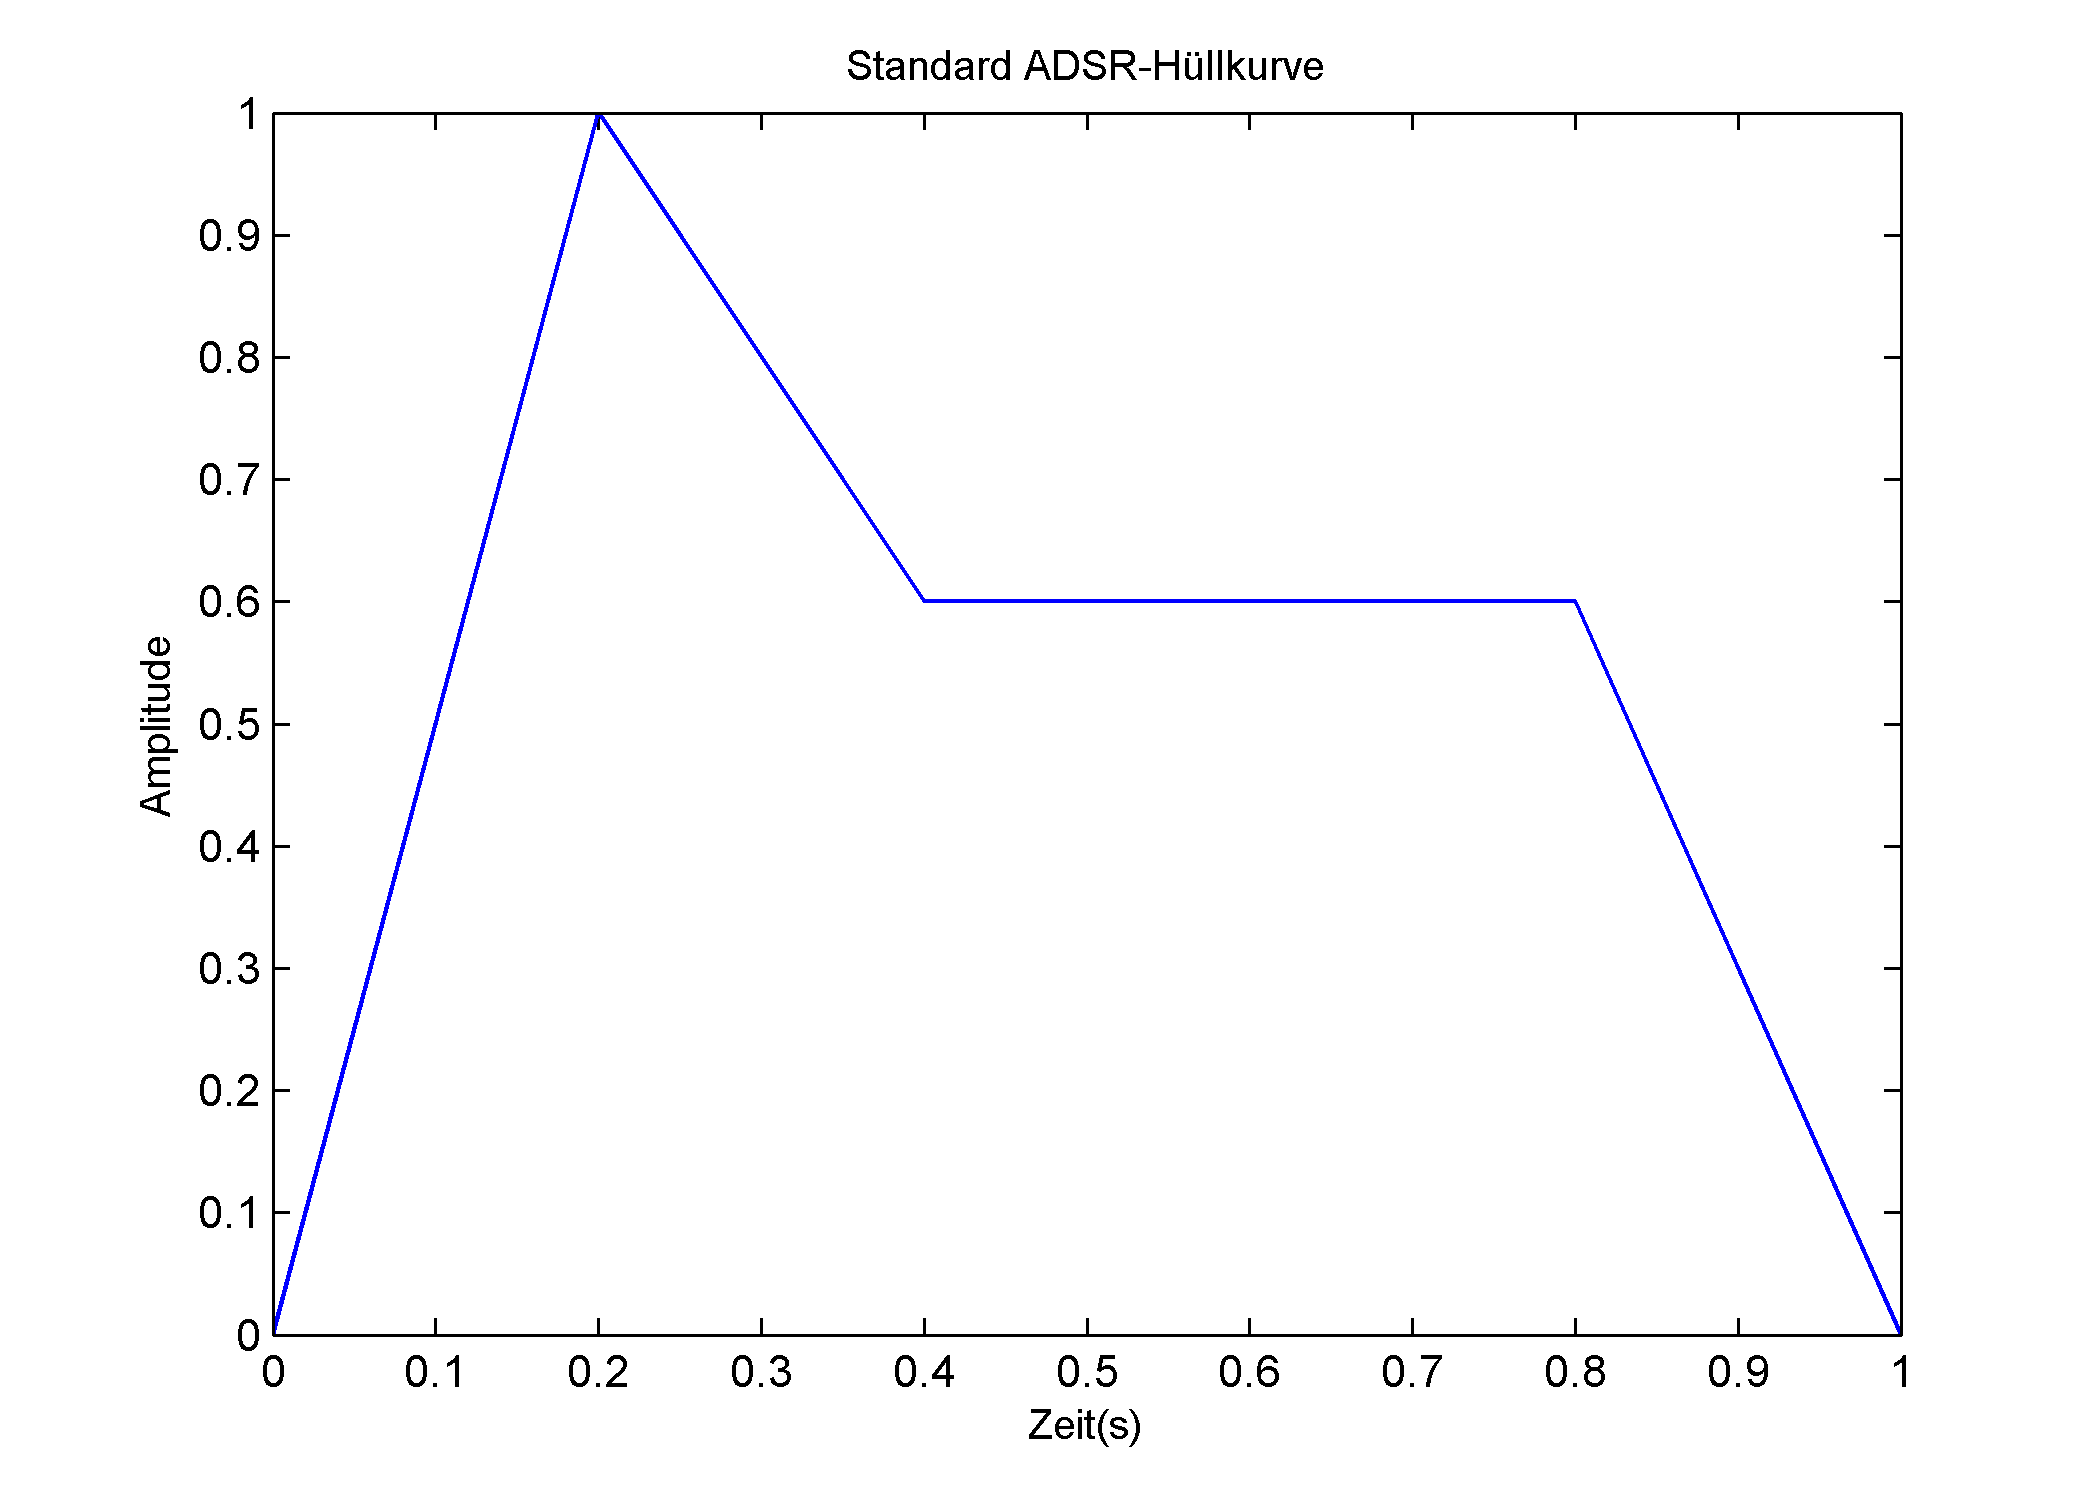
\includegraphics[width=0.5\textwidth]{adsrDefault.png}
\caption{Standard ADSR-Hüllkurve}
\label{fig:adsrDefault}
Quelle: Eigene Darstellung mit Matlab
\end{figure}

Da allerdings bei vielen Instrumenten die Lautstärke in den einzelnen Phasen der ADSR-Hüllkurve nicht gleichmäßig steigt oder sinkt, ist es nötig die Kurven beliebig Komplex abbilden zu können. Bei vielen Instrumenten steigt beispielsweise die Lautstärke in der Attack Phase exponentiell an und fällt in der Decay und Release Phase auch wieder exponentiell ab. Manche Synthesizer bieten zusätzlich auch noch eine Hold Phase vor der Attack Phase, da es Instrumente gibt, die einige Zeit benötigen bis sie nach dem Anschlagen des Tones in die Attack Phase eintreten. In Abbildung \ref{fig:adsrTypical} wurden weitere für Instrumenten typische Hüllkurven dargestellt um zu verdeutlichen, dass die ADSR-Hüllkurve bei Instrumenten beliebig komplexe Formen annehmen kann.

\begin{figure} [ht]
\centering
  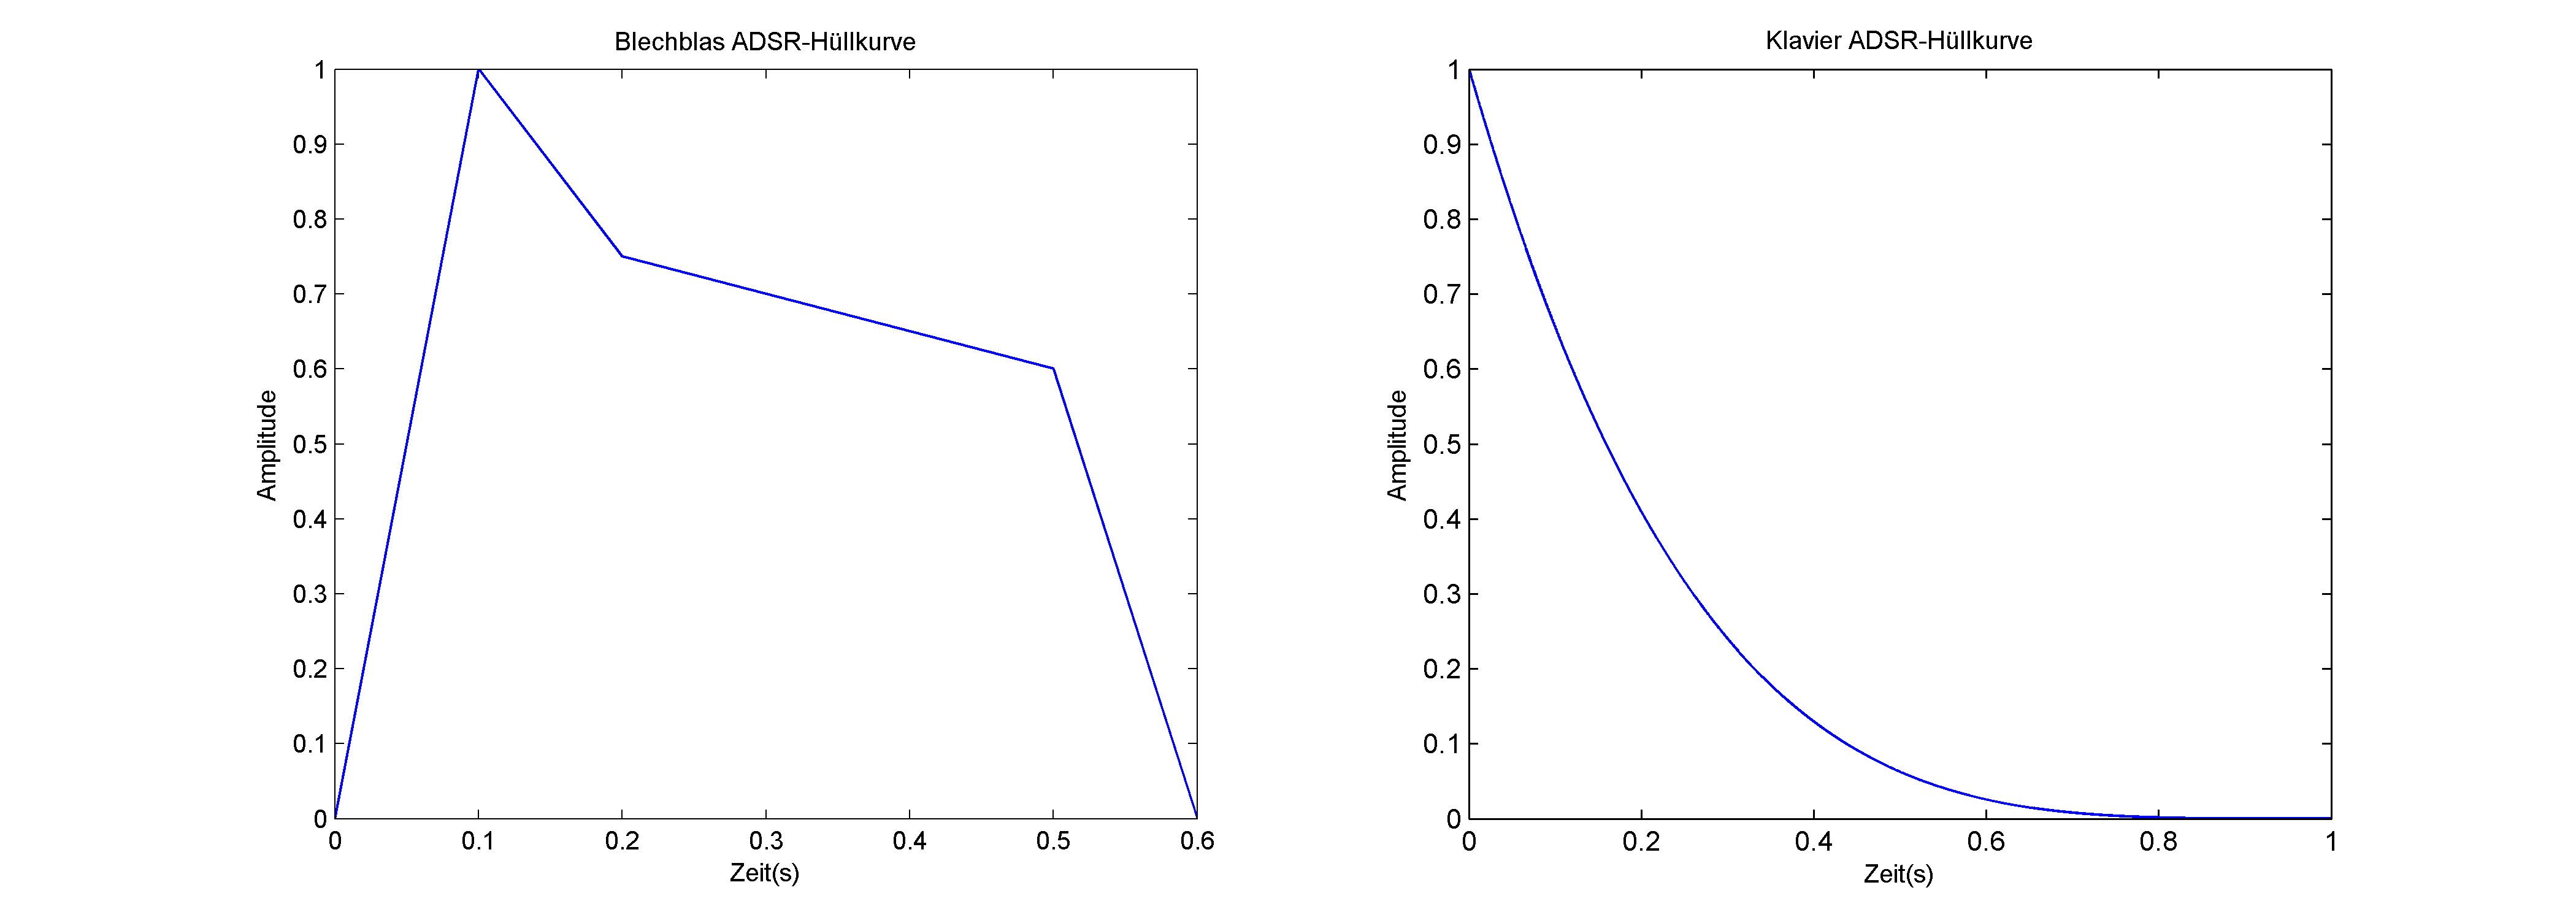
\includegraphics[width=1\textwidth]{adsrTypical.png}
\caption{Typische ADSR-Hüllkurve eines Blechblasinstrumentes und eines Klaviers}
\label{fig:adsrTypical}
Quelle: Eigene Darstellung mit Matlab
\end{figure}

Auch wenn das Hinzufügen einer ADSR-Hüllkurve den Klang des synthetisierten Tones schon natürlicher wirken lässt, hört sich der erzeugte Ton leider noch nicht wie ein echtes Instrument an. Eine weitere Möglichkeit ihn zu verbessern, stellt die Varrierung des Modulationsindex über die Zeit oder die Amplitude dar. Somit kann die Anzahl der Seitenfrequenzen verändert werden, was zu einem lebendigeren Klang führt. Bei Blasinstrumenten wird der Modulationsindex typischerweise über die Amplitude (also mit der ADSR-Hüllkurve) variiert. \cite[S. 532]{chowningPaper}

Eine weitere Möglichkeit den Klang des Tones zu verbessern stellen Filter dar. Filter können genutzt werden um das von der FM Synthese erzeugte Signal zu manipulieren. Dabei werden ungewollte Frequenzen gedämpft bzw. komplett heraus gefiltert. Typische Vertreter von Filtern sind Hochpassfilter, Tiefpassfilter, Bandpass und Bandsperre. \cite[S. 100-104]{stotz}

Das bisher erzeugte Signal ist noch ein reines Signal, welches so in der Natur nicht vorkommen kann. Bei Luftverwirblungen und Unebenheiten des Instrumentes tritt Rauschen auf. Dieses Rauschen trägt zum typischen Klangbild eines Instrumentes bei und sollte auch nachgebildet werden. Ein Rauschen kann mittels Feedback-FM-Synthese erzeugt werden, dafür muss der Modulationsindex der Feedback-FM-Synthese sehr hoch angesetzt werden. Das von der Feedback-FM-Synthese erzeugte Signal gleicht bei sehr hohem Modulationsindex einem weißen Rauschen. Anschließend kann dieses Rauschen mittels Multibandpassfilter um die jeweiligen ausgeprägten Frequenzen gefiltert werden. Würde das Rauschen nicht gefiltert werden, kann neben dem Ton, das Rauschen als solches wahrgenommen werden. [TODO CITE]

Um den Klang des Synthetisierten Tones noch natürlicher zu gestalten, könnte dem Ton noch ein Hall-Effekt hinzugefügt werden.


\FloatBarrier
\subsubsection{Nachbildung eines Tones einer Querflöte mittels FM-Synthese}

Im Laufe dieses Kapitels soll ein Ton einer Querflöte mittels FM-Synthese erzeugt und mit den oben beschriebenen Techniken verfeinert werden. Alle Beispiele sind in Matlab erstellt und können mit den beiliegenden Dateien nachgestellt werden. In Abbildung \ref{fig:plotFluteOrig} sind Spektrogram, Waveform und Spektrum des originalen Querflöten Tones abgebildet. Mit den Information aus den vorliegenden Grafiken wird versucht, diesen spezifischen Ton nachzubilden.

\begin{figure} [h!t!b!]
\centering
  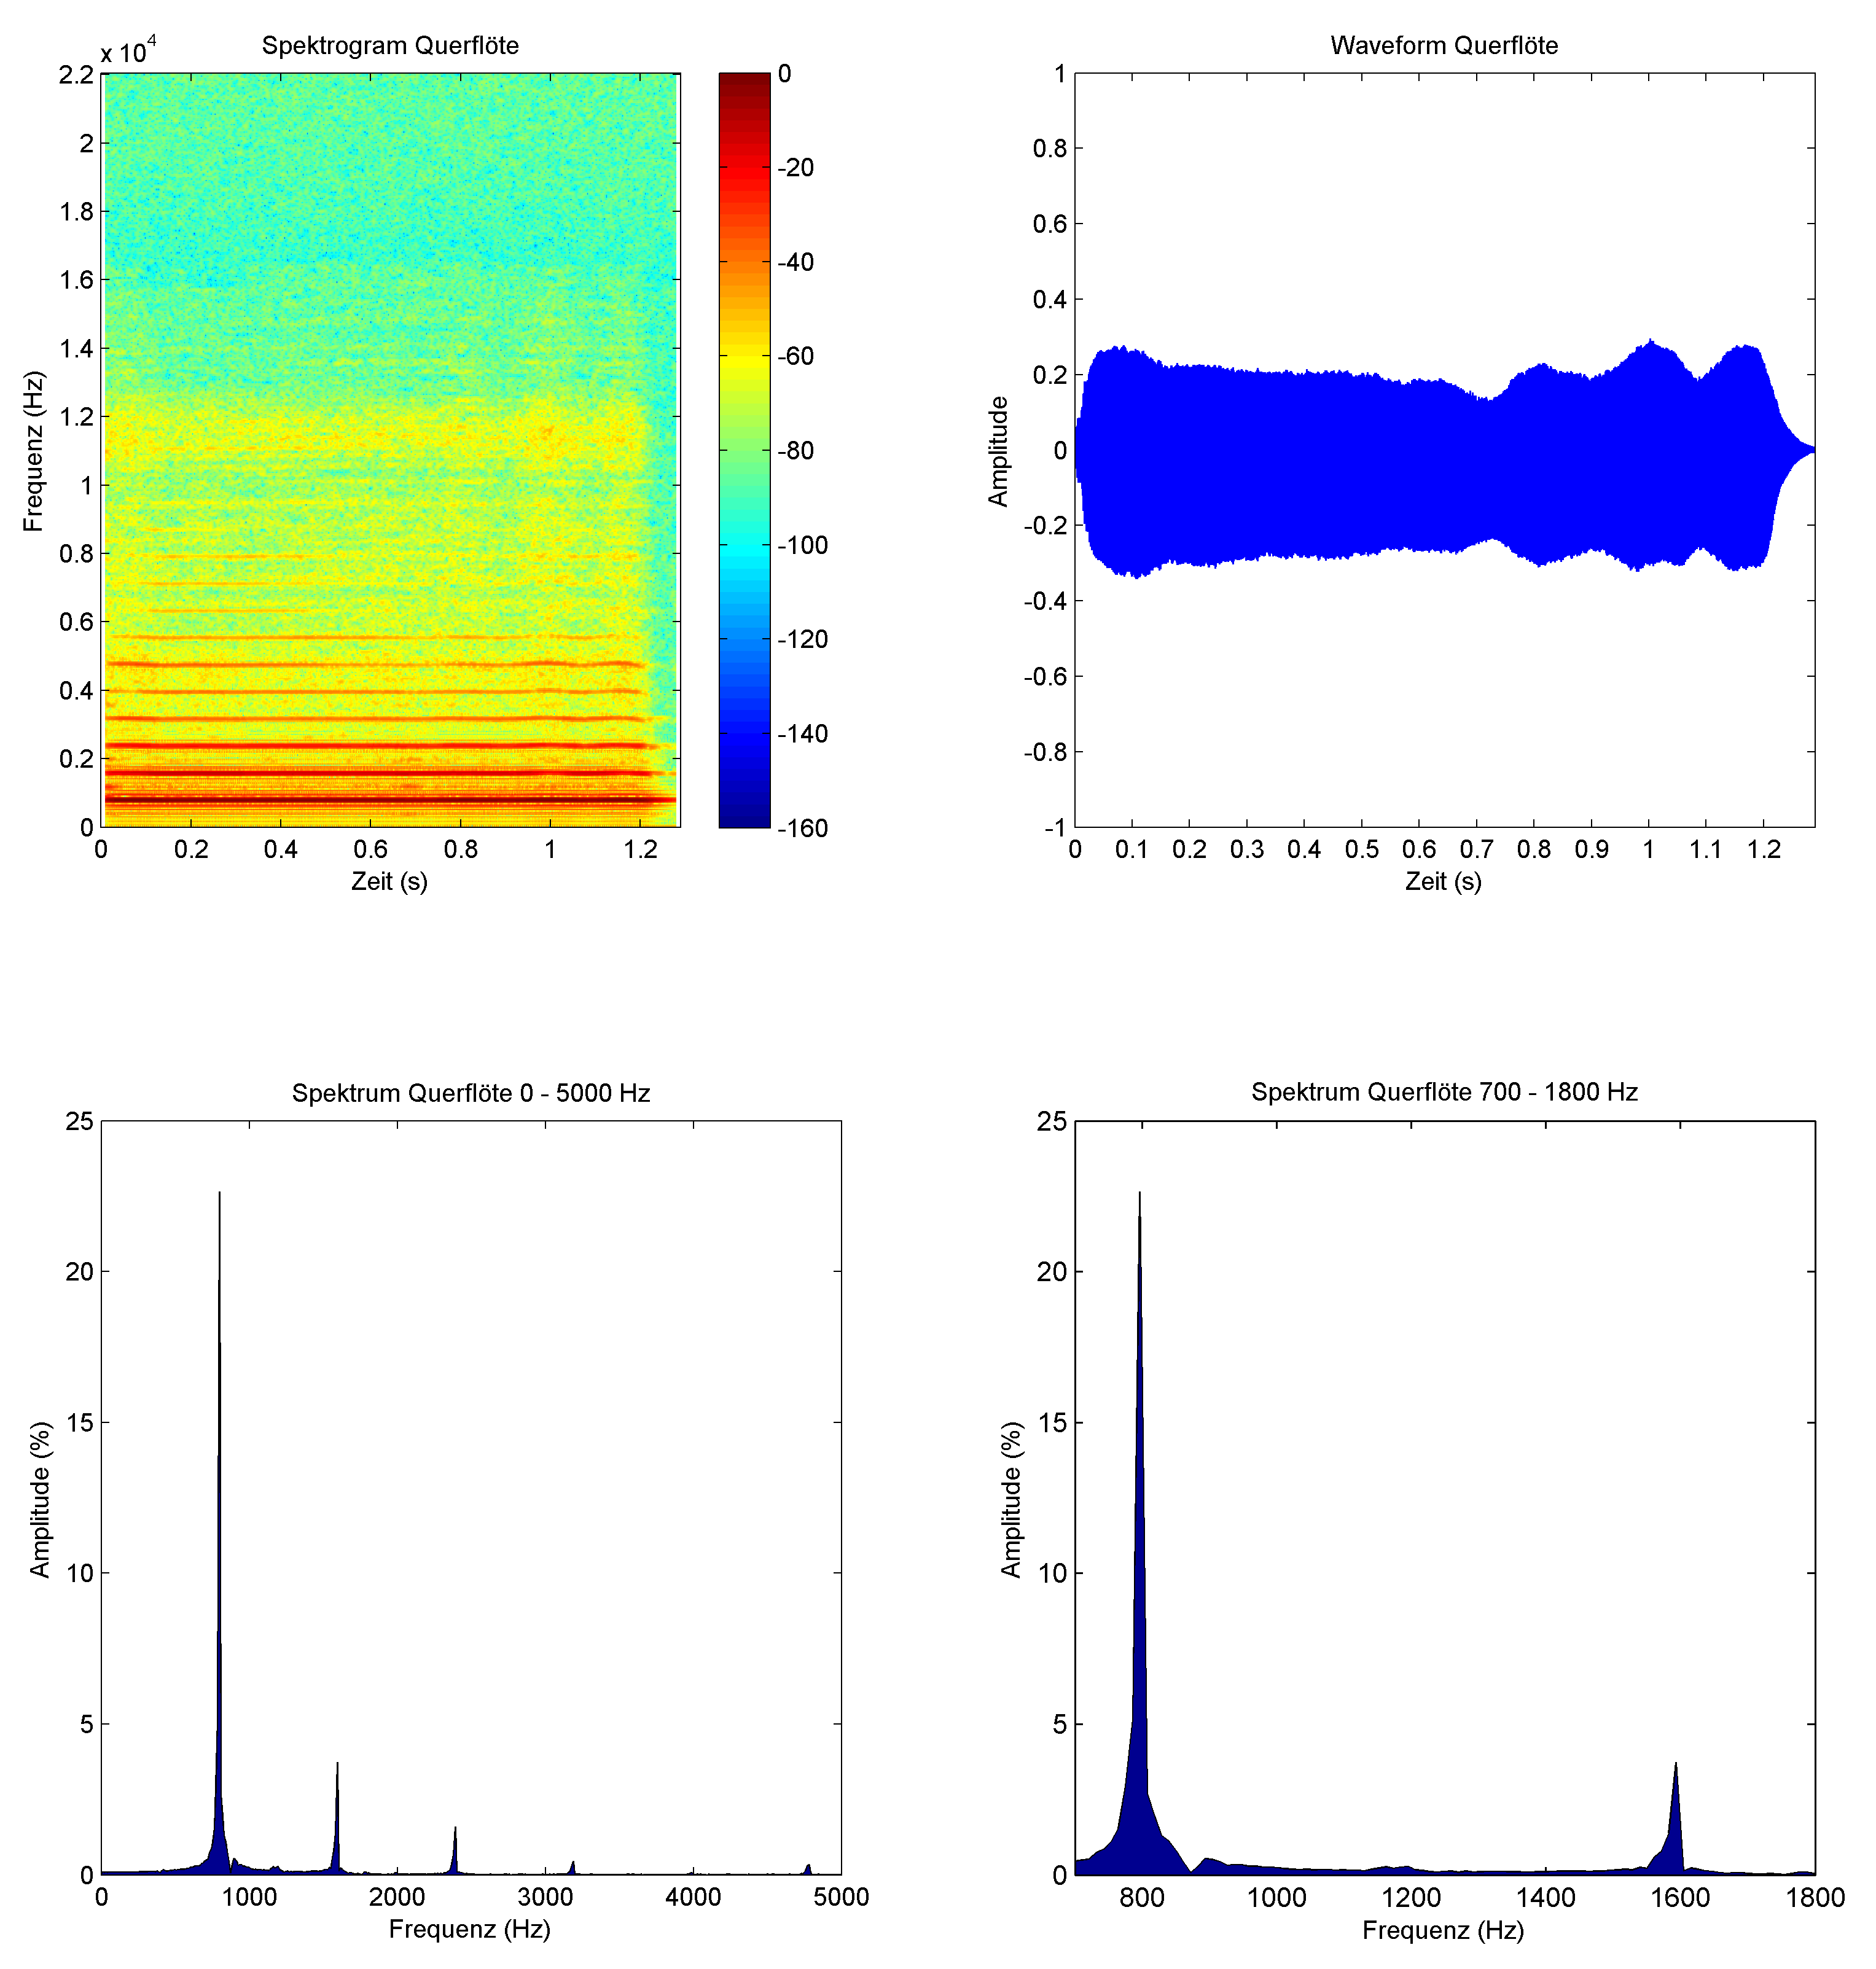
\includegraphics[width=1\textwidth]{plotFluteOrig.png}
\caption{Plot des Spektrograms, der Waveform und des Spektrums eines echten Tones einer Querflöte}
\label{fig:plotFluteOrig}
Quelle: Eigene Darstellung mit Matlab
\end{figure}

Anhand des Spektrums können bereits einige Erkenntnisse für die FM-Synthese ausgelesen werden. Zunächst ist zu bemerken, dass die am stärksten ausgeprägte Frequenz bei etwa 800 Hz liegt. Bei genauerer Betrachtung wird sichtbar, dass die Frequenz nicht exakt bei 800 Hz sondern bei 796.75 Hz ihren maximalen Ausschlag erreicht. Dies entspricht am ehesten einem G5 mit 784 Hz \cite[S. 181]{borucki}. Diese Frequenz (796.75 Hz) werden wir bei der FM-Synthese als Träger Frequenz nutzen. Im Spektrum sind außerdem noch mehrere Seitenfrequenzen zu sehen. Die erste dieser Seitenfrequenzen befindet sich bei etwa dem doppelten der Grundfrequenz. Bei genauerer Betrachtung wird sichtbar das sie ihren maximalen Amplitudenwert wirklich genau bei dem doppeltem der Grundfrequenz (1593.5 Hz) hat. Also ist der Abstand zwischen Grundfrequenz und erster Seitenfrequenz genauso groß wie der Abstand von 0 Hz bis zur Grundfrequenz, hierbei ist zu bemerken, dass der Abstand von einem ganzzahligen Multiplikator mit der Grundfrequenz typisch für einen harmonischen Ton ist \cite[S. 528]{chowningPaper}. Die nächsten Seitenfrequenzen haben jeweils wieder den selben Abstand von 796.75 Hz zur jeweiligen vorangegangenen Seitenfrequenz. Aus dieser Beobachtung können wir unsere Modulationsfrequenz von 796.75 Hz schließen. Anhand der Anzahl der sichtbaren Seitenfrequenzen im Spektrum können wir eine ungefähre Abschätzung unseres Modulationsindexes wagen. Somit wird als Modulationsindex für die ersten Tests vorerst 0.5 angenommen. 

\begin{figure} [ht]
\centering
  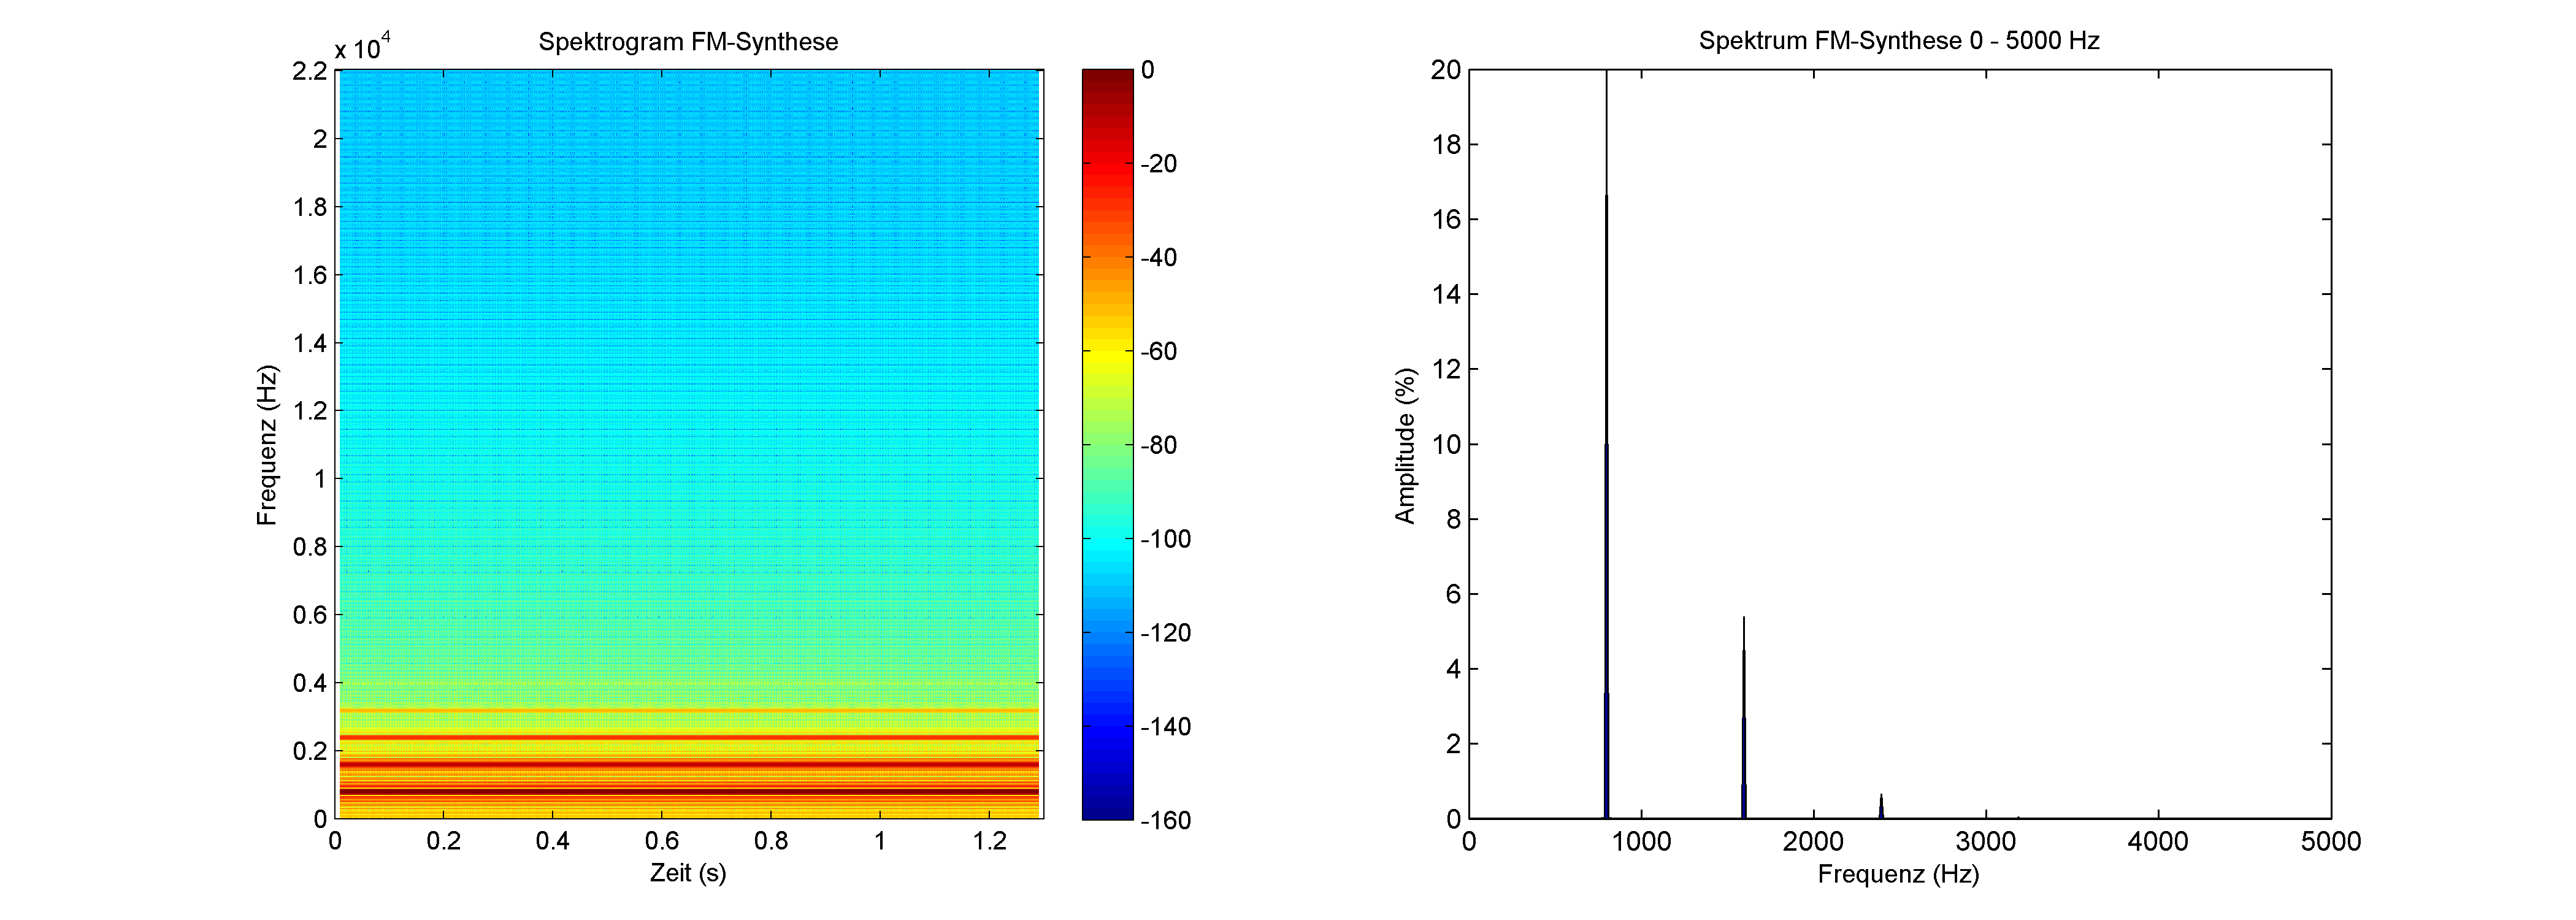
\includegraphics[width=1\textwidth]{plotFMSyntheseI05.png}
\caption{Plot des Spektrograms und des Spektrums der FM-Synthese mit den Parametern fc = 796.75 Hz, fm = fc und I = 0.5 }
\label{fig:plotFMSyntheseI05}
Quelle: Eigene Darstellung mit Matlab
\end{figure}

Ein erstes Spektrum der FM-Synthese mit den eben festgelegten Werten kann in Abbildung \ref{fig:plotFMSyntheseI05} begutachtet werden. Beim Evaluieren der Ergebnisse dieses Spektrums fällt auf, dass die erste Seitenfrequenz im Verhältnis zur Grundfrequenz einen viel Stärkeren Ausschlag aufweist als es bei der Querflöte der Fall ist. Außerdem fällt danach die Amplitude der 2. und 3. Seitenfrequenz viel stärker ab als bei dem Instrument. Sieht man sich jetzt noch das Spektrogram (ebenfalls in Abbildung \ref{fig:plotFMSyntheseI05}) an, fällt im Vergleich zum Spektrogram der Querflöte die sehr viel geringer Anzahl an Seitenfrequenzen auf. Die Seitenfrequenzen bei 4000 Hz und darüber sind bei dem Instrument noch deutlich sichtbar während sie bei der FM-Synthese schon bei 4000 Hz kaum noch existent sind. Versucht man jetzt den Modulationsindex zu erhöhen um die Anzahl der Seitenfrequenzen zu erhöhen, verlagert sich die Amplitude unserer Trägerfrequenz auf die Seitenfrequenzen, damit werden die Seitenfrequenz stärker und die Träger Frequenz schwächer, zu sehen in Abbildung \ref{fig:spektrumFMSyntheseI2}. 

\begin{figure} [ht]
\centering
  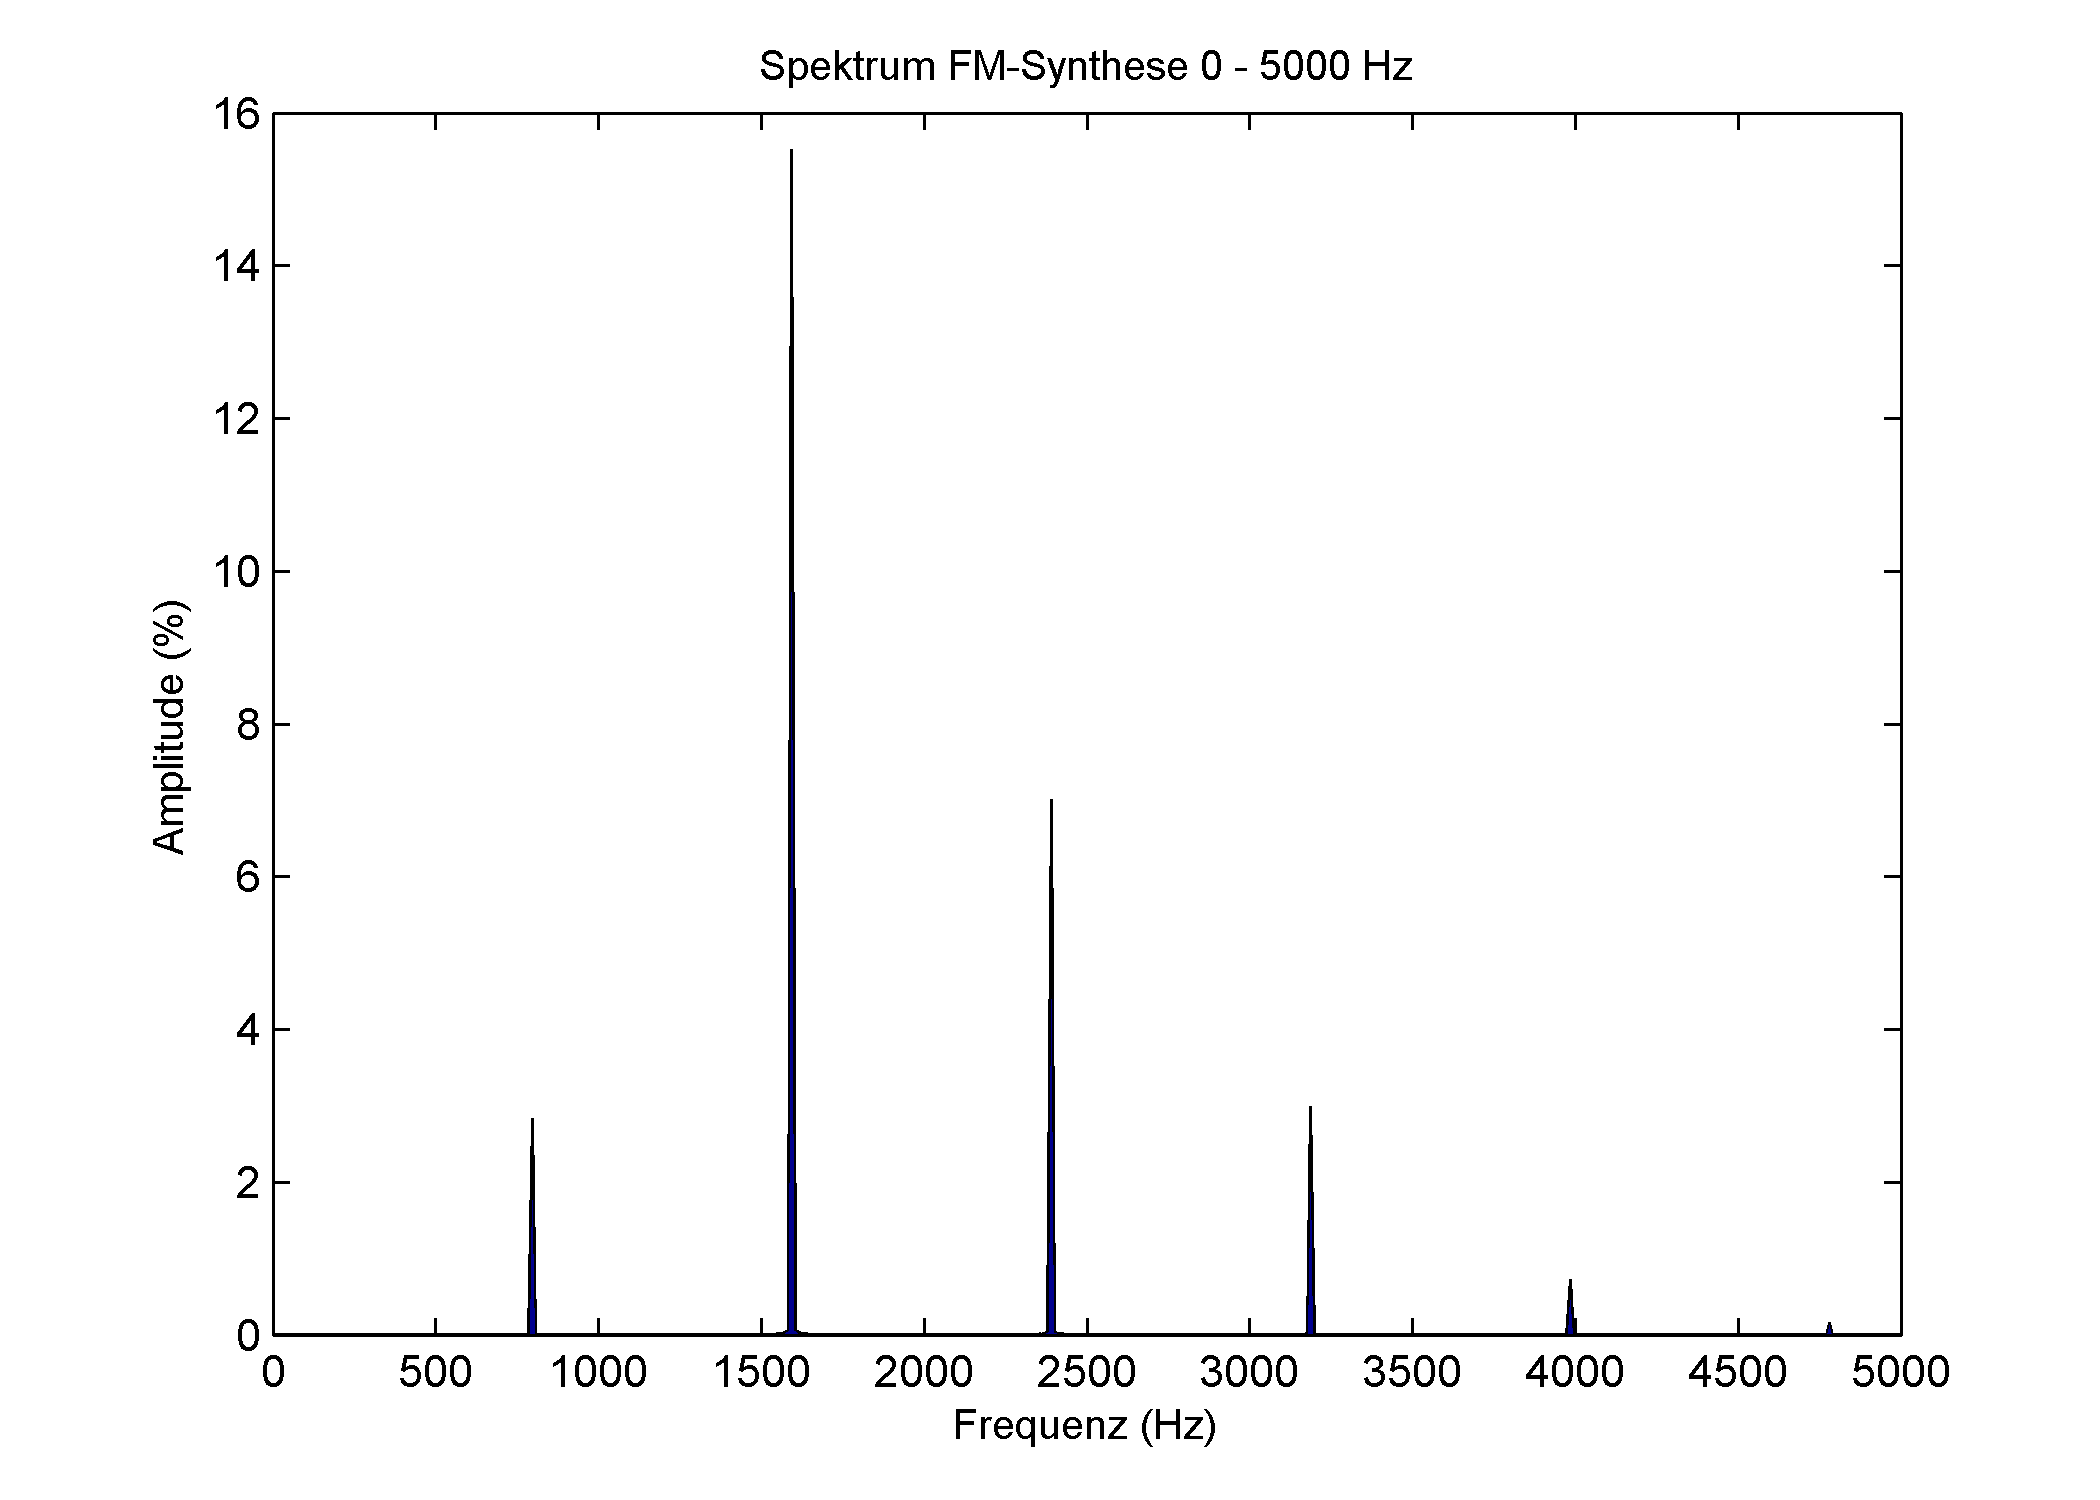
\includegraphics[width=0.5\textwidth]{spektrumFMSyntheseI2.png}
\caption{Plot des Spektrums der FM-Synthese mit den Parametern fc = 796.75 Hz, fm = fc und I = 2}
\label{fig:spektrumFMSyntheseI2}
Quelle: Eigene Darstellung mit Matlab
\end{figure}

Um dieses Verhalten zu umgehen müssen wir uns der Komplexen FM-Synthese widmen. Hier werden mehrere Modulatoren verschachtelt um eine größere Anzahl an Seitenfrequenzen zu erzeugen. Allerdings ist es bei der Komplexen FM-Synthese schwer vorauszusagen wie stark die Amplituden der einzelnen Seitenfrequenzen ausgeprägt sind, deshalb braucht es hier einige Experimente um auf das gewünschte Ergebnis zu stoßen. In Abbildung \ref{fig:plotFMSyntheseKomplex4Mod} sehen sie das Ergebnis der FM-Synthese mit 4 Modulatoren. Dieses Spektrum ähnelt dem der Querflöte schon sehr viel stärker und auch das Spektrogram weißt in den Intensitäten der Seitenfrequenzen eine deutliche Ähnlichkeit auf.

\begin{figure} [ht]
\centering
  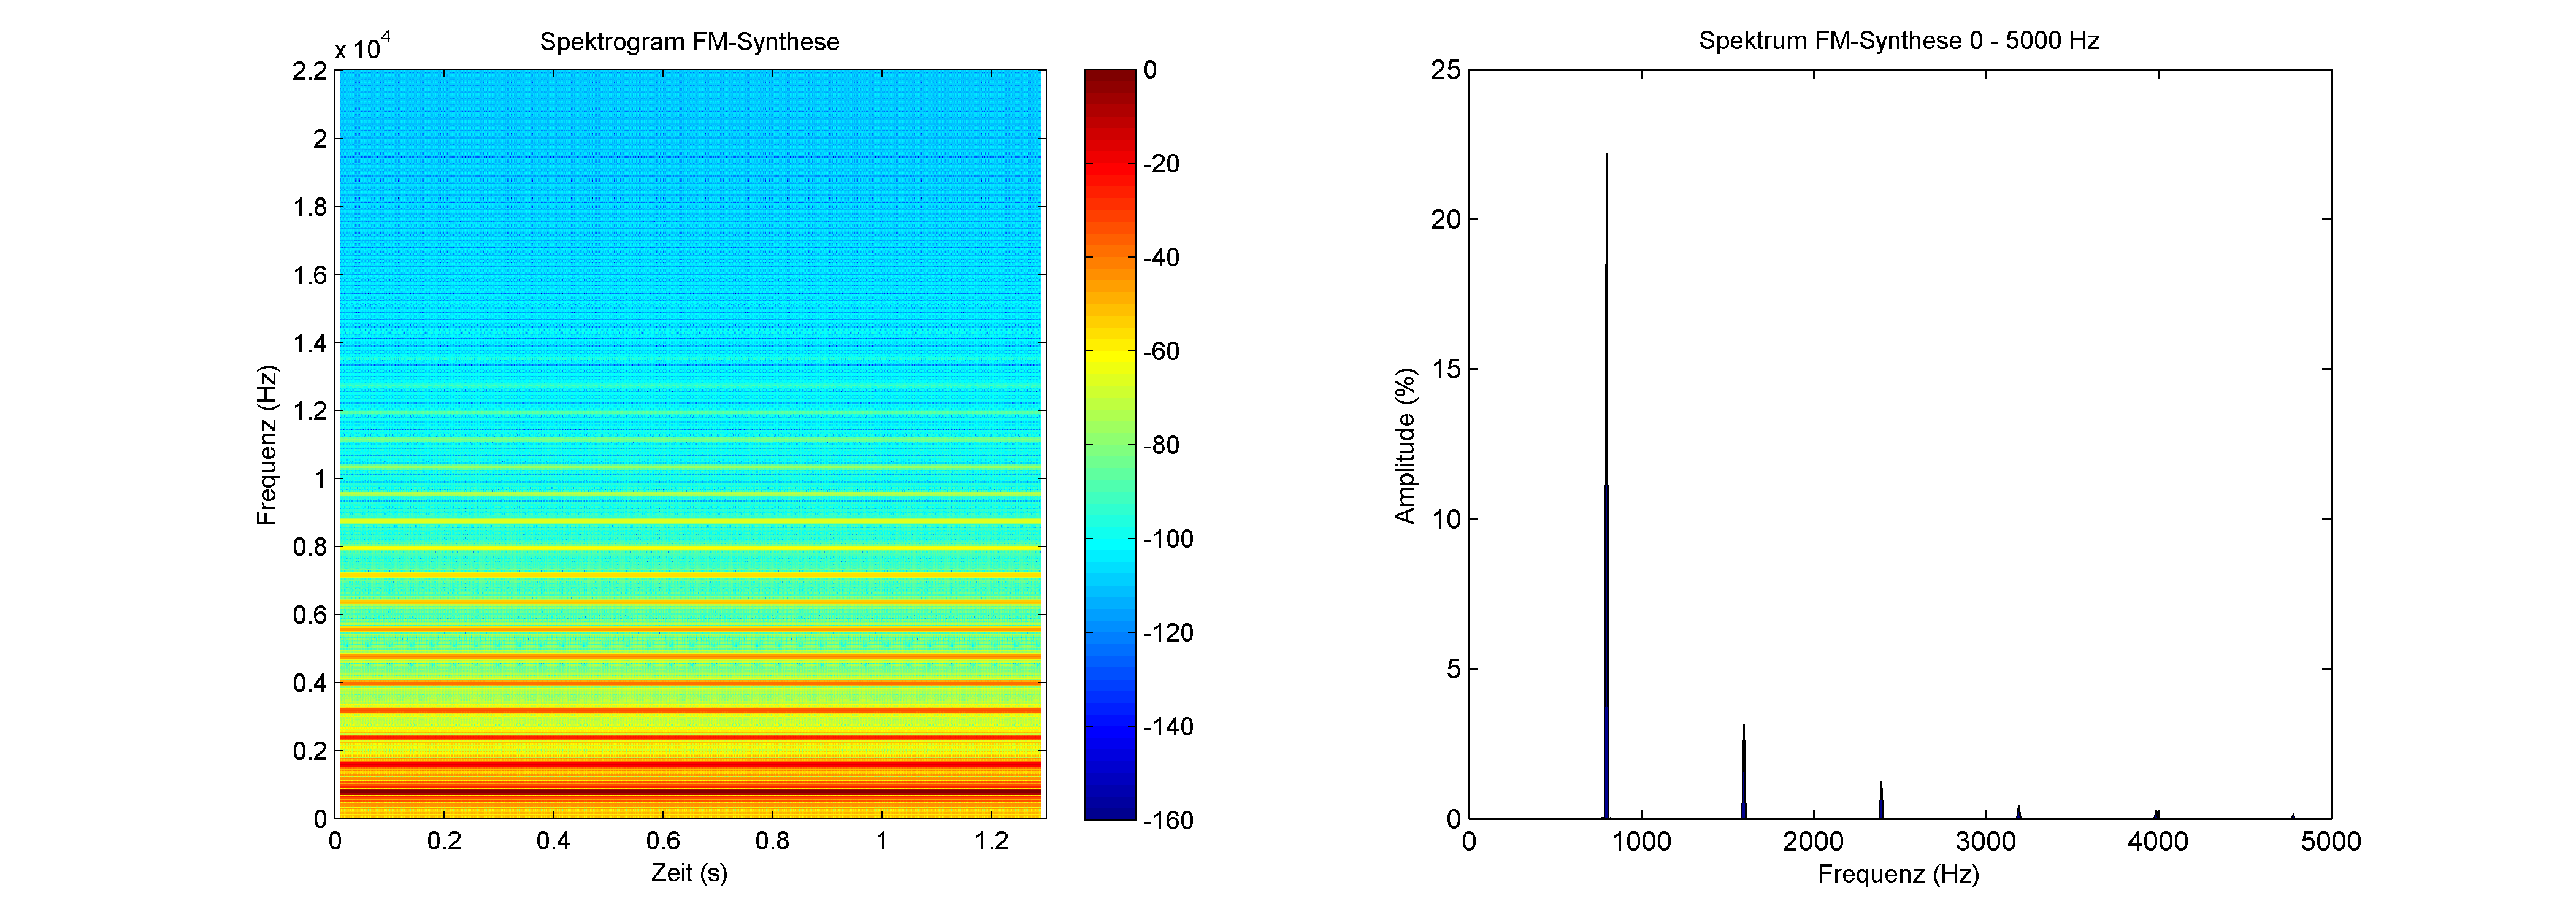
\includegraphics[width=1\textwidth]{plotFMSyntheseKomplex4Mod.png}
\caption{Plot des Spektrograms und des Spektrums der FM-Synthese mit 4 Modulatoren und den Parametern fc = 796.75 Hz, fm1 = fm2 = fm3 = fm4 = fc, I1 = 0.3, I2 = 0.5, I3 = 1 und I4 = 1}
\label{fig:plotFMSyntheseKomplex4Mod}
Quelle: Eigene Darstellung mit Matlab
\end{figure}

Da die Grundeinstellung der FM-Synthese mit den oben genannten Parametern ein zufriedenstellendes Signal erzeugt, können wir uns jetzt der Veredlung des Tones widmen. Zuerst wird dem Signal ein Vibrato hinzugefügt. Durch das Hinzufügen des Vibratos, schwingt der erzeugte Ton leicht und wirkt lebendiger und nicht ganz so künstlich. Dies kann bewerkstelligt werden indem die Modulationsfrequenz leicht erhöht oder verringert wird. Auch hierbei muss experimentiert werden, welche Erhöhung der Modulationsfrequenz das gewünschte Ergebnis erzeugt. Als sehr ähnlich zum Original Ton hat sich in diesem Fall eine Erhöhung um 2.5 Hz herausgestellt. Unsere neue Modulationsfrequenz ist somit fm = fc + 2.5. In Abbildung \ref{fig:spektrumFMSyntheseVibrato} wird die Auswirkung des Vibratos sichtbar, es bilden sich um die Seitenfrequenzen weitere recht gering ausgeprägte Frequenzausschläge.

\begin{figure} [ht]
\centering
  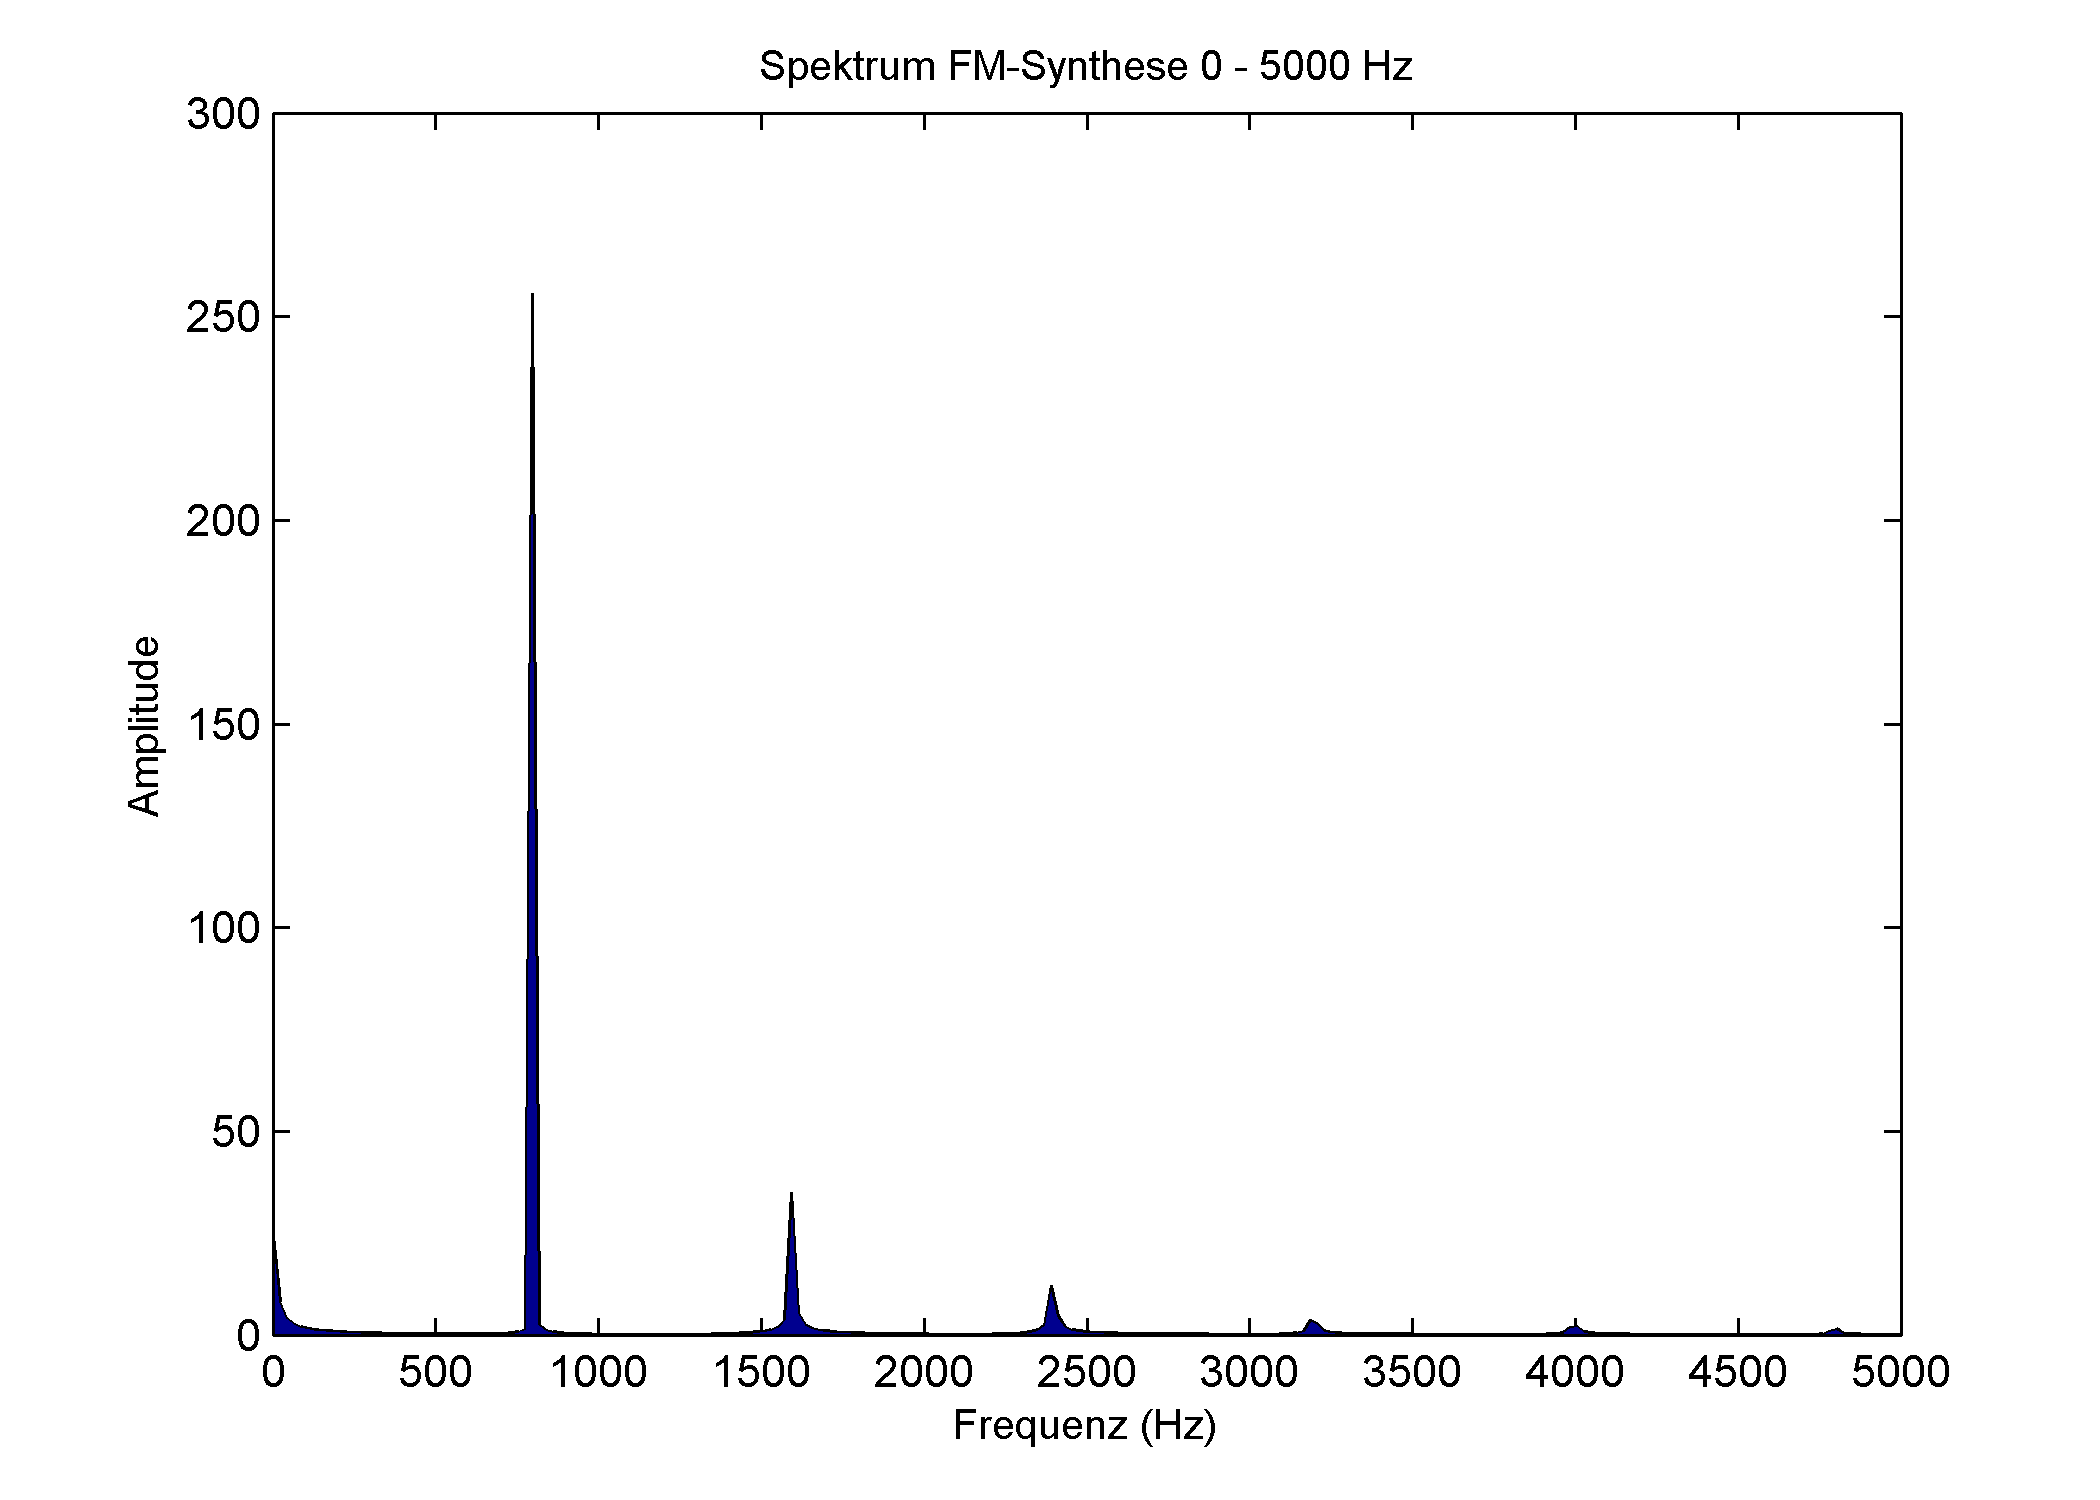
\includegraphics[width=0.5\textwidth]{spektrumFMSyntheseVibrato.png}
\caption{Plot des Spektrums der FM-Synthese mit 4 Modulatoren, Vibrato und den Parameter fc = 796.75 Hz, fm1 = fm2 = fm3 = fm4 = fc +2.5, I1 = 0.3, I2 = 0.5, I3 = 1 und I4 = 1}
\label{fig:spektrumFMSyntheseVibrato}
Quelle: Eigene Darstellung mit Matlab
\end{figure}

Der nächste wichtige und einfach hinzuzufügende Bestandteil des synthetisierten Tones ist die ADSR-Hüllkurve. Um generell eine Querflöte nachzumachen wäre eine Hüllkurve wie in Abbildung \ref{fig:adsrFlute} links gezeigt möglich. Allerdings versuchen wir den originalen Ton der Querflöte so gut wie möglich nachzuahmen, hierfür wurde eine Komplexere Hüllkurve nach dem Beispiel der Waveform des original Tones generiert. Bei dieser Hüllkurve wurde Attack, Decay und Release von der Allgemeinen Hüllkurve übernommen und die Sustain Phase angepasst, zu sehen in Abbildung \ref{fig:adsrFlute} rechts. 

\begin{figure} [ht]
\centering
  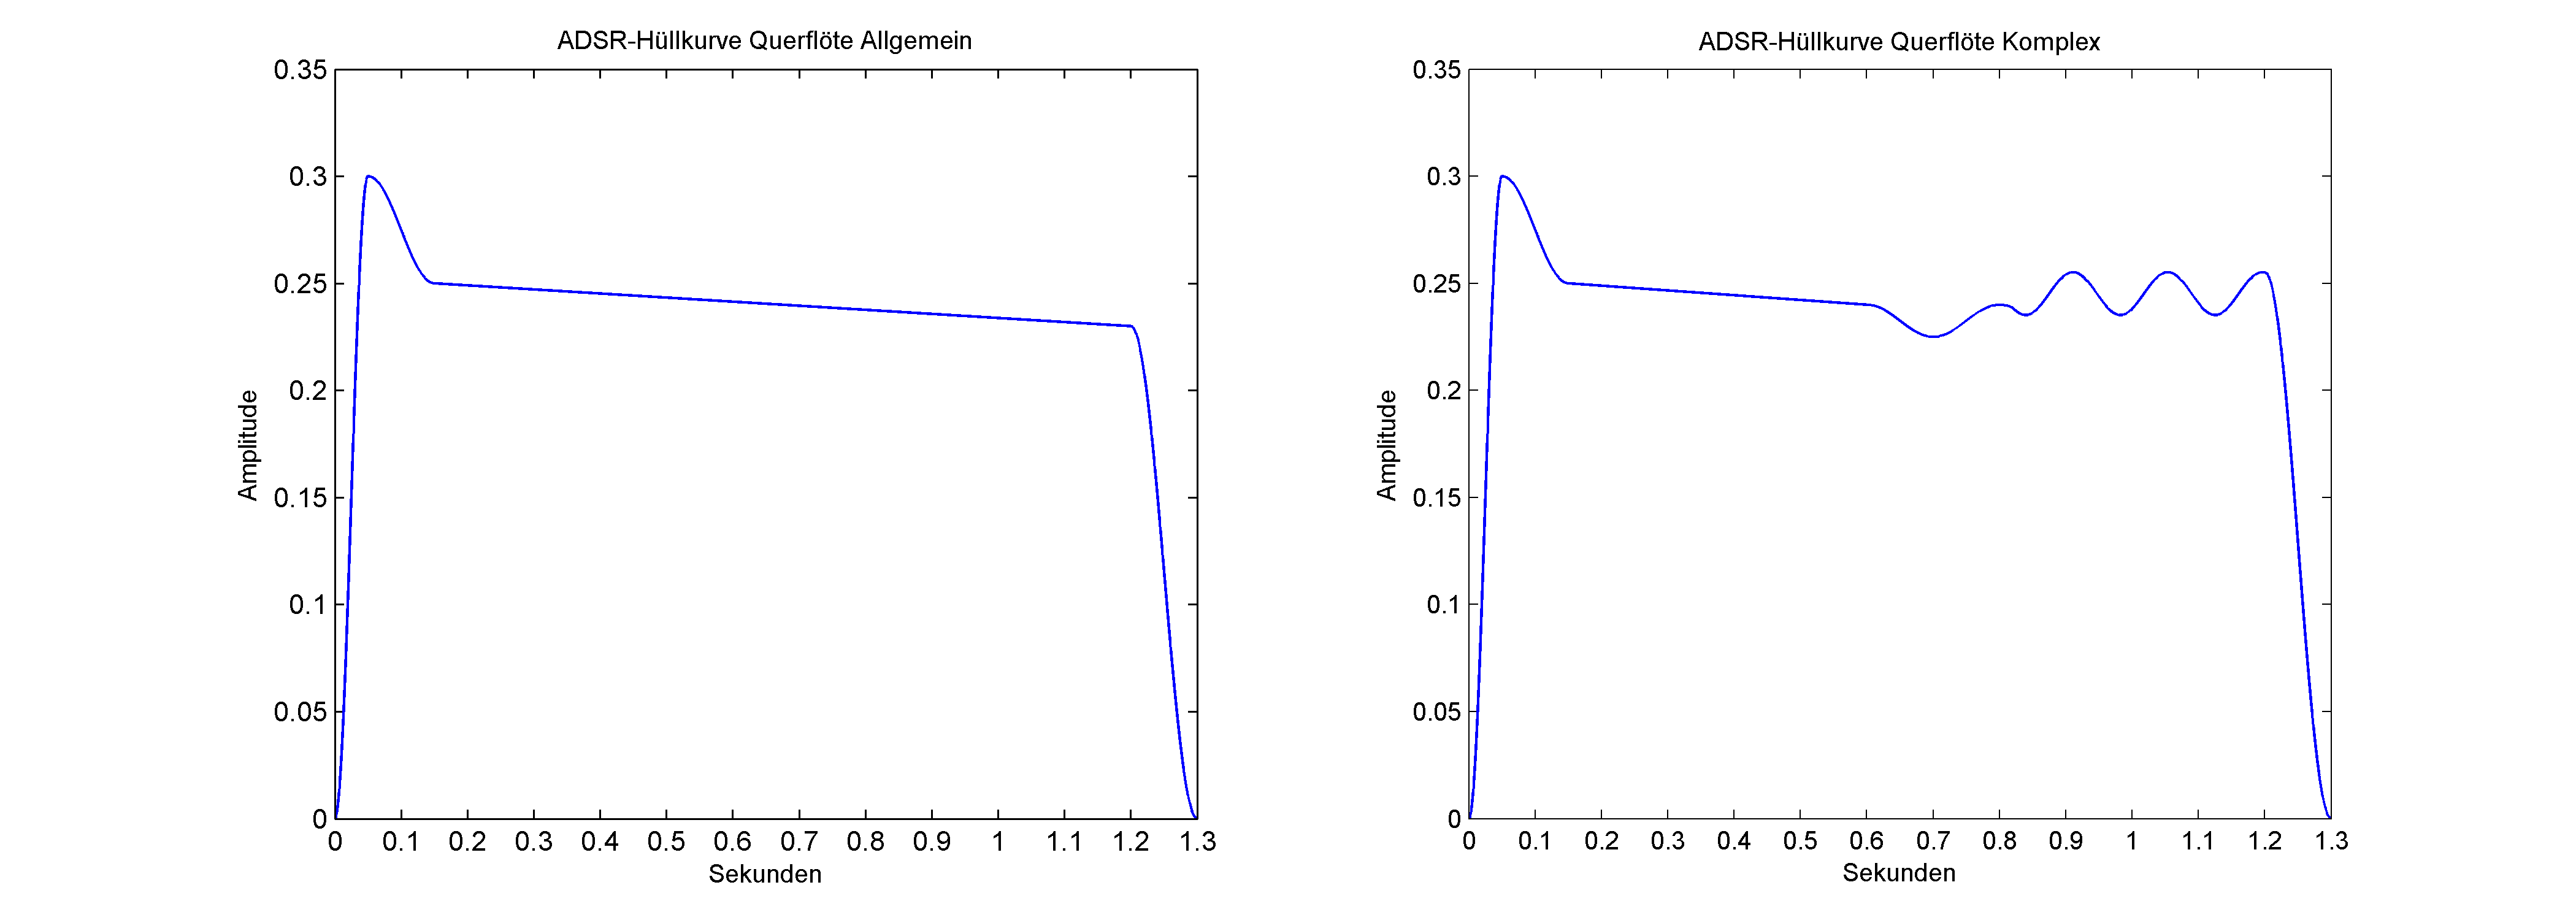
\includegraphics[width=1\textwidth]{adsrFlute.png}
\caption{Plot der ADSR-Hüllkurve einer Querflöte und der hier genutzten, komplexeren Hüllkurve}
\label{fig:adsrFlute}
Quelle: Eigene Darstellung mit Matlab
\end{figure}

Nachdem die ADSR-Hüllkurve hinzugefügt wurde, fällt im Spektrogram auf, dass die Seitenfrequenzen trotz geringerer Amplitude bei Attack und Release Phase einen größeren Ausschlag als beim Instrument aufweist. Dieser Ausschlag kann verringert werden, indem der erste Modulationsindex mit der ADSR-Hüllkurve variiert wird. 

Nachdem Vibrato, Variabler Modulationsindex und ADSR-Hüllkurve hinzugefügt wurden, hat sich das Spektrogram zur Abbildung \ref{fig:plotFMSyntheseKomplex4Mod} kaum geändert. Es wird nur der Vibrato durch die etwas breiteren Seitenfrequenzen und die ADSR-Hüllkurve durch ansteigen des Spektrums zu Beginn des Tones und Abfallen des Spektrums nach 1.2 Sekunden sichtbar. Der Ton hört sich von der Tonhöhe und der Intensität schon stark nach dem Originalen Querflötenton an. Allerdings fehlen noch die Typischen Blas- und Luftverwirblungsgeräusche sowie das sehr starke Anblasgeräusch. Um die typischen Blasgeräusche zu erzeugen wird zunächst ein Rauschen mittels FM Feedback Generator mit hohem Modulationsindex erzeugt. Würde das Rauschen ohne weitere Arbeitsschritte dem synthetisiertem Signal hinzugefügt, könnte das Rauschen stark herausgehört werden. Um dies zu verhindern muss das Rauschen vorerst gefiltert werden. Hierzu wird ein Multibandpassfilter über alle möglichen Seitenfrequenzen erstellt. Das Gefilterte Rauschen wird anschließend noch mit einer ADSR-Hüllkurve veredelt. Dieser Schritt ist nötig, da während der Attack-Phase des Original Tones, wie im Spektrogram in Abbildung \ref{fig:plotFluteOrig} zu sehen, das Rauschen durch das Anblasen des Instrumentes sehr scharf heraus sticht. Zusätzlich kann noch ein sehr leises Rauschen des Feedback-FM-Generators ohne Filter über das ganze Frequenzspektrum gelegt werden um auch in den höheren Frequenzen einen leichten Ausschlag im Spektrogram kenntlich zu machen. Trotz des verstärkten Rauschens zu Begin des Tones, fehlt noch der Starke hörbare Ton der dabei entsteht. Beim betrachten des Spektrums und des Spektrograms fallen noch 2 recht Starke Ausschläge zu Begin des Signals auf. Ein Ausschlag befindet sich bei 904.3 Hz und der zweite bei 1182 Hz. Beide Frequenzen können mit einem einfachen Sinus erzeugt und mit einer ADSR-Hüllkurve, die nur eine kurze Attack-Phase aufweist, modeliert und zum Signal addiert werden. In Abbildung \ref{fig:spektrogramFMSyntheseComplete} ist das Ergebnis der FM-Synthese mit den, in diesem Kapitel, besprochenen Veredelungen gezeigt. In den Plots sind die Ähnlichkeiten zum originalen Ton deutlich zu sehen.

\begin{figure} [h!t!b!]
\centering
  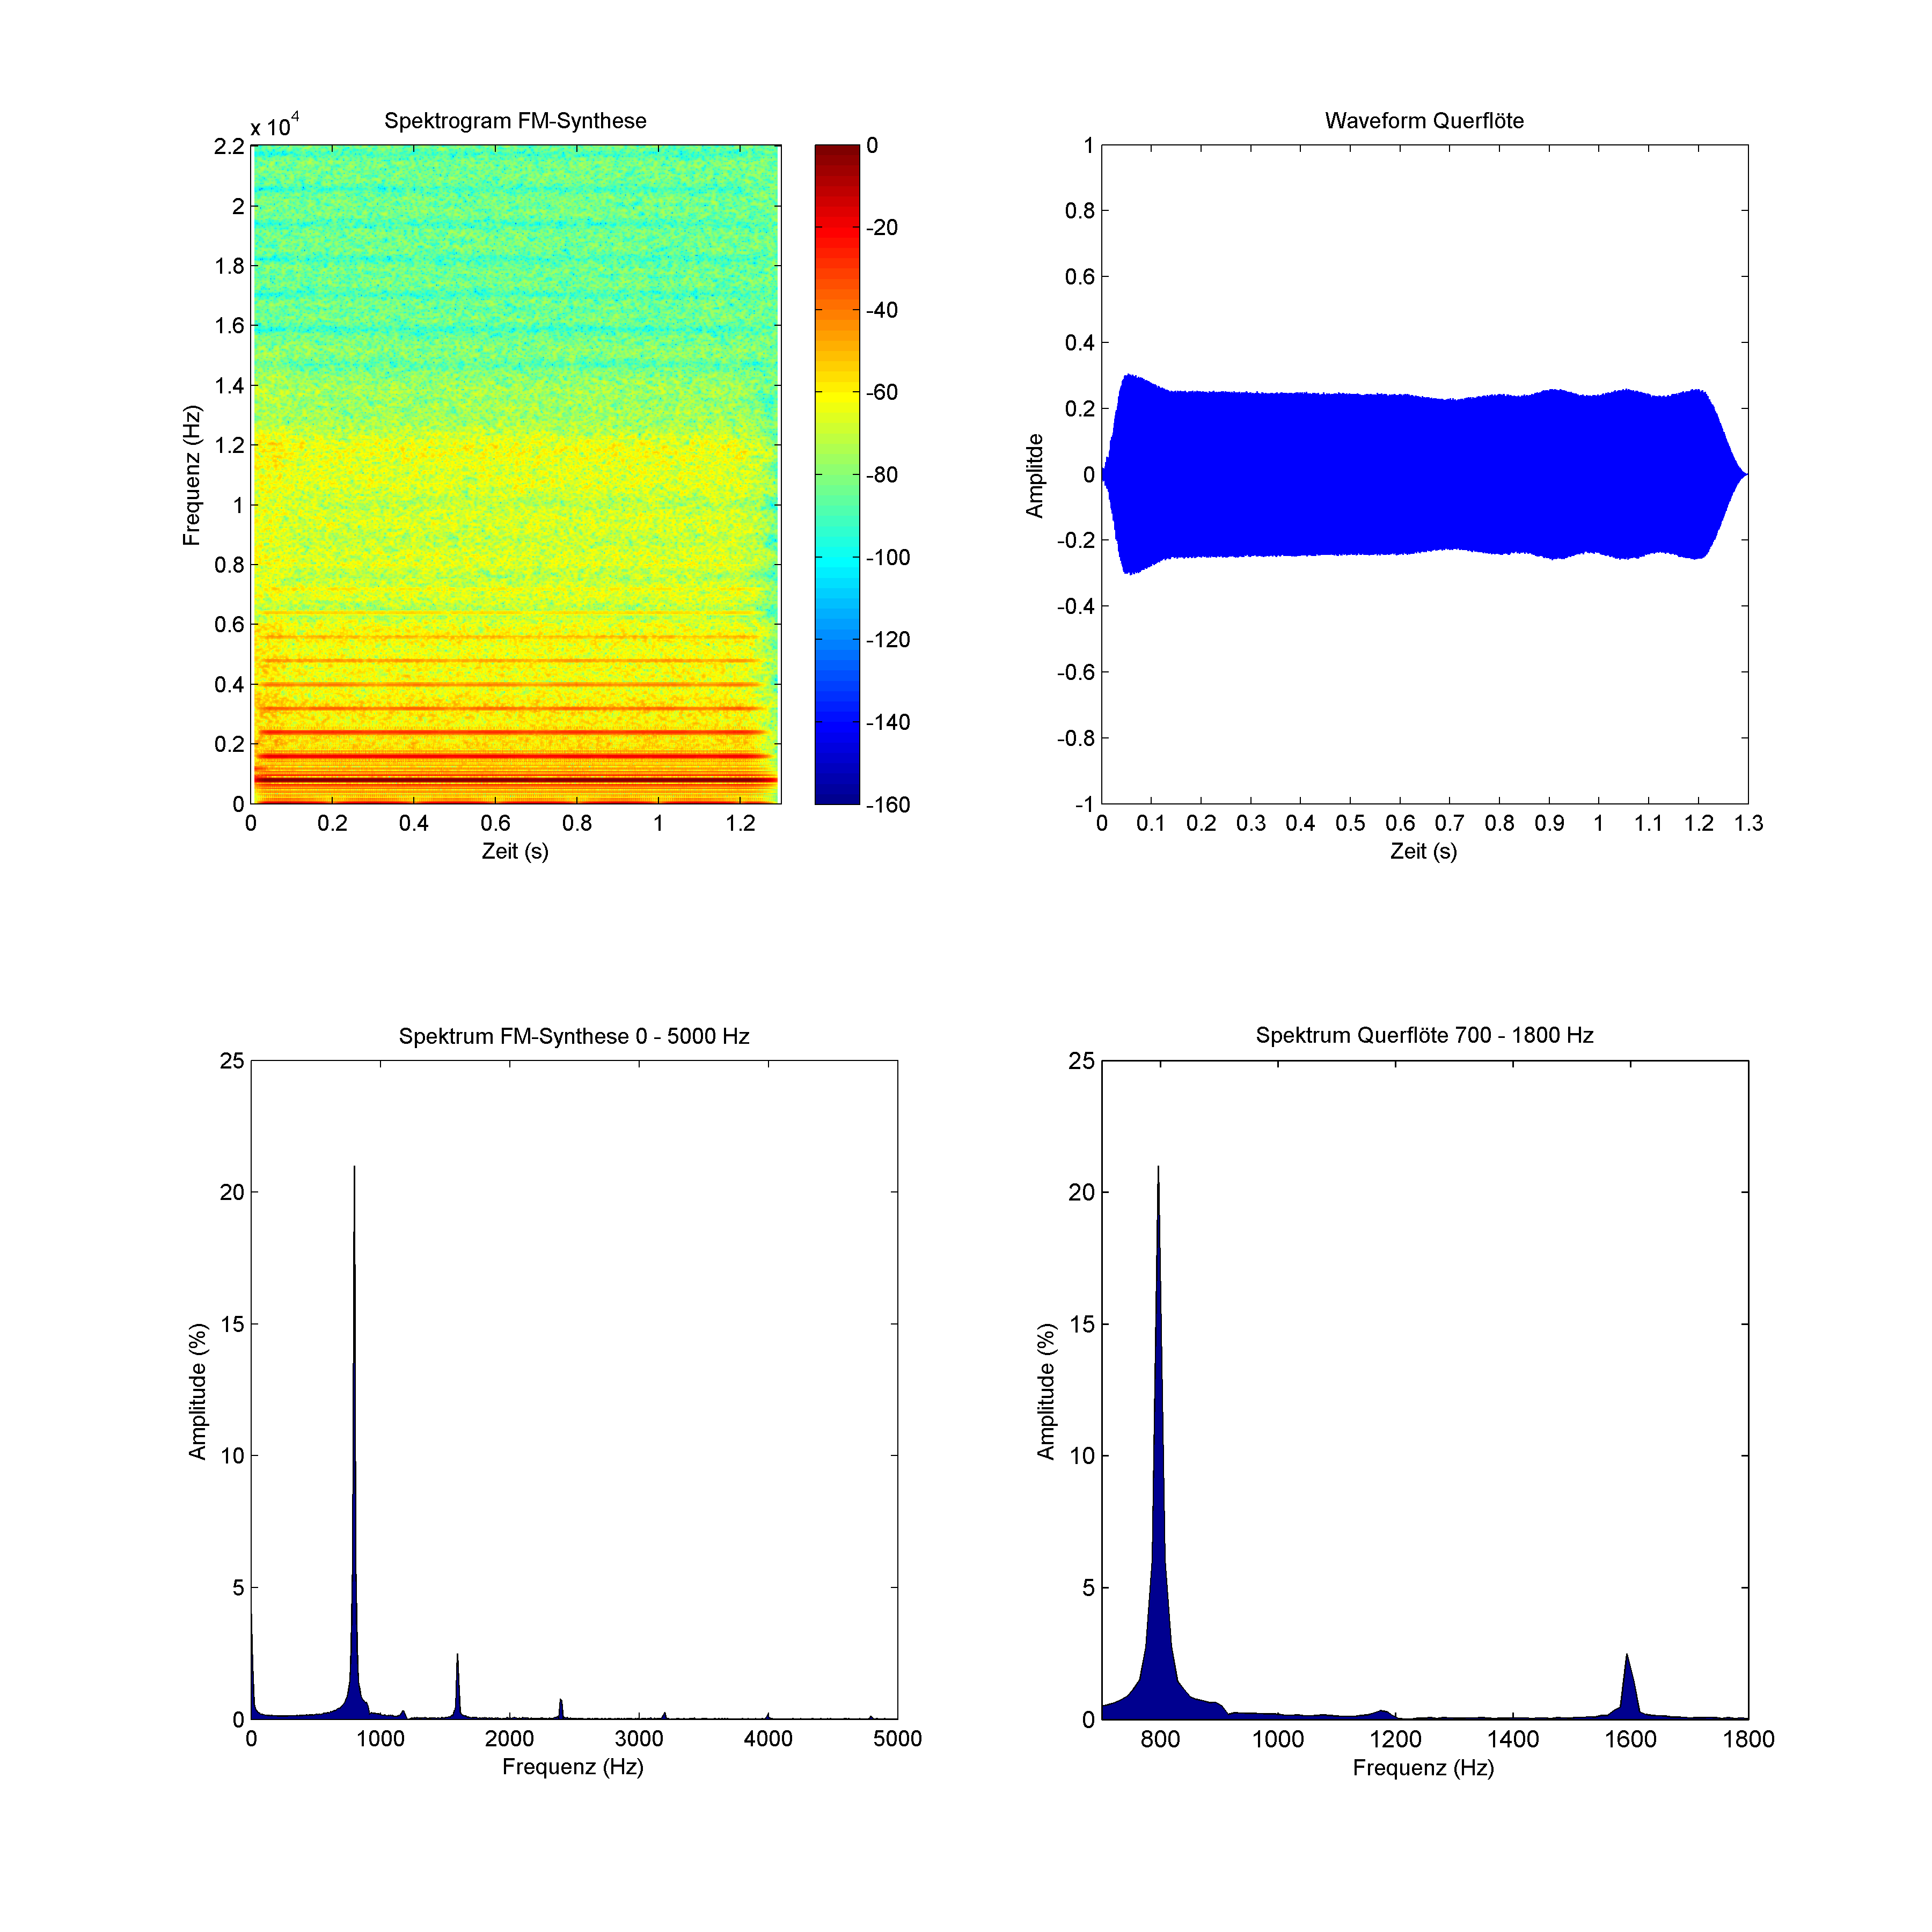
\includegraphics[width=1\textwidth]{spektrogramFMSyntheseComplete.png}
\caption{Plot des fertigen Tones der FM-Synthese mit 4 Modulatoren, ADSR-Hüllkurve, Variablem Modulationsindex, Vibrato, Rauschen und Anblasgeräusch}
\label{fig:spektrogramFMSyntheseComplete}
Quelle: Eigene Darstellung mit Matlab
\end{figure}

Der in diesem Kapitel synthetisierte Ton gleicht dem originalen Flöten Ton sehr stark. Trotzdem weißt der Flöten Ton noch etwas mehr Lebendigkeit auf, da das gesamte Signal nicht so statisch wie das, der FM-Synthese ist. 

Dieses Ergebnis zeigt, dass es sehr wohl möglich ist, wenn auch mit erheblichem Aufwand verbunden, mit der FM-Synthese einen natürlich wirkenden Instrumententon zu erzeugen. Gerade in diesem Beispiel fällt allerdings auf das der synthetisierte Ton im Vergleich zum originalen Ton nicht ganz so lebendig empfunden wird. Das hängt in diesem Fall vorallem an der nicht sehr neutralen Spielweise des Querflötenspielers.


\FloatBarrier
\subsubsection{FM Parametrisierung mittels Genetischer Algorithmen}

Mittels genetischer Algorithmen ist es möglich Parameter der FM Synthese herauszufinden, die nötig sind um einen Ton zu erzeugen der einem echten Instrument nachempfunden ist. Diese Algorithmen zerlegen einen echten Ton eines Instrumentes mittels Schneller Fourier Transformation in seine einzelnen Bestandteile und versucht verschiedene Parameter für die Synthese aus, zerlegt das entstandene Signal wieder mittels Schneller Fourier Transformation und vergleicht die Ergebnisse. Mit diesem Verfahren können recht zuverlässig realistisch Synthetisierte Töne erzeugt werden, die von einem Originalen Instrument kaum zu unterscheiden sind. Da für die Implementierung eines solchen Algorithmus allerdings die Zeit fehlt, wird dieses Thema in dieser Arbeit nicht weiter vertieft. Eine Ausführliche Erklärung der FM Parametrisierung mittels Genetischer Algorithmen kann in Andrew Horners Artikel "Nested Modulator and Feedback FM Matching of Instrument Tones" nachgelesen werden.

\FloatBarrier
\subsection{Modulationsframework (Theorie -> Praxis)}
\FloatBarrier
\subsection{Demo: Parameter und Effekte - Grafiken (evtl. Plotten)}

\section{Praxis}

\subsection{Do-It-Yourself (Projekt hochladen, Kopfhörer!)}

\section{Fazit}

Chownings Entdeckung führte zu einer Revolution des Synthesizer Marktes. Der DX7 von Yamaha war einer der erfolgreichsten Synthesizer und trug maßgeblich zu dieser Revolution bei. Obwohl die zugrundeliegende Formel simpel wirkt, sind die mathematischen Hintergründe nicht trivial. Durch komplexe Anordnung von Trägern und Modulatoren können beliebig komplexe Klänge erzeugt werden. Dies führt zu einer mächtigen, jedoch wenig intuitiven Technik. Musiker können durch Experimentieren verschiedener Parametern und Konfigurationen interessante Klänge erzeugen. Außerdem kann die FM-Synthese dazu verwendet werden, um ganze Instrumente nachzubilden.
Wie in dieser Arbeit gezeigt wurde, ist dies bei sorgfältiger Ausnutzung der Eigenschaften von einfacher und komplexer FM-Synthese sowie unter Wahl der geeigneten Parametern mit einem gewissen Maß an Erfindungsreichtum sehr gut zu bewerkstelligen.

\bibliography{seminar}

\end{document}